% --------------------------------------------------------------------
% Preamble
% --------------------------------------------------------------------
\documentclass[paper=a4, fontsize=11pt,twoside]{scrartcl}   

\usepackage[a4paper,pdftex]{geometry}   
\setlength{\oddsidemargin}{5mm}           
\setlength{\evensidemargin}{5mm}

\usepackage[english]{babel}
\usepackage[protrusion=true,expansion=true]{microtype}    
\usepackage{amsmath,amsfonts,amsthm,amssymb}
\usepackage{algorithm}
\usepackage[noend]{algpseudocode}
\usepackage{float}
\usepackage{listings}

%\usepackage[draft]{graphicx}
\usepackage{graphicx}
\usepackage{setspace}
\usepackage{hyperref}
\usepackage{ragged2e}
\usepackage{tabto}
\usepackage{afterpage}
\usepackage[usenames, dvipsnames]{color}
\usepackage{titlesec}
\usepackage{lipsum}
\usepackage{tipa}
\usepackage{amsthm}
\usepackage{relsize}
\usepackage{color}
\usepackage{chngcntr}
\usepackage{textcomp}
\usepackage[binary-units=true]{siunitx}
\numberwithin{table}{section}
\numberwithin{figure}{section}
\numberwithin{algorithm}{section}
\usepackage{url}


% --------------------------------------------------------------------
% Definitions
% --------------------------------------------------------------------
\newcommand{\HRule}[1]{\rule{\linewidth}{#1}}     

\makeatletter                            
\def\printtitle{%                        
    {\centering \@title\par}}
\makeatother                                    

\makeatletter                           
\def\printauthor{%                    
    {\large \@author}}                
\makeatother       

\newcommand\blankpage{%
    \null
    \thispagestyle{empty}%
    \addtocounter{page}{-1}%
    \newpage}                     

\definecolor{mygray}{gray}{0.6}

\titleformat{\section}
{\normalfont\huge\bfseries}
{\thesection\hskip 12pt\textcolor{mygray}{\textdoublepipe}\hskip 20pt}
{0pt}
{}

\titlespacing*{\section}{0pt}{18pt}{13pt}

\newtheorem{ddef}{Definition}[section]


\definecolor{mygreen}{rgb}{0,0.6,0}
\definecolor{mygray}{rgb}{0.5,0.5,0.5}
\definecolor{mymauve}{rgb}{0.58,0,0.82}

\lstset{language=C++}
\lstset{
  backgroundcolor=\color{white},   % choose the background color
  basicstyle=\footnotesize,        % size of fonts used for the code
  breaklines=true,                 % automatic line breaking only at whitespace
  captionpos=b,                    % sets the caption-position to bottom
  commentstyle=\color{mygreen},    % comment style
  escapeinside={\%*}{*)},          % if you want to add LaTeX within your code
  keywordstyle=\color{blue},       % keyword style
  stringstyle=\color{mymauve},     % string literal style
  morekeywords={uint32_t, int32_t},
  literate={~} {$\sim$}{1},
}


% --------------------------------------------------------------------
% Metadata
% --------------------------------------------------------------------

\title{
	\begin{flushright}
		\LARGE{\textit{Scott Williams}}
	\end{flushright}
	~\\[2.0cm]			
	\normalsize \textsc{Computer Science Part II Project Dissertation}\\[2.0cm]     
    \HRule{0.5pt} \\                        
    \LARGE \textbf{\uppercase{Steganographic file systems within video files}}    
    \HRule{2pt} \\[30pt]        
    \normalsize Christ's College\\[5pt]University of Cambridge\\[25pt]           
    \normalsize \today            
}

\author{
    \begin{spacing}{1.5}
        \noindent
        \uppercase{Project Supervisor}: Daniel Thomas\\    
        \uppercase{Director of Studies}: Professor Ian Leslie\\    
        \uppercase{Project Overseers}: Professor Peter Robinson, Dr Robert Watson\\
    \end{spacing}
}


\begin{document}
\renewcommand{\thelstlisting}{\thesection.\arabic{lstlisting}}
\counterwithin{lstlisting}{section}
% ------------------------------------------------------------------------------
% Maketitle
% ------------------------------------------------------------------------------
\thispagestyle{empty}        

\printtitle                    
\vfill
\begin{center}
\huge{[~}\normalsize \textsc{First Draft}\huge{~]}
\end{center}
\afterpage{\blankpage}
\newpage
% ------------------------------------------------------------------------------
% Begin document
% ------------------------------------------------------------------------------
\setcounter{page}{1}        
\pagenumbering{roman}
\section*{Performa}
\NumTabs{3}
\textsc{Name}: \tab{Scott Williams}\\
\textsc{College}: \tab{Christ's}\\
\textsc{Project Title}: \tab{Steganographic file systems within video files}\\
\textsc{Examination}: \tab{Part II of the Computer Science Tripos}\\
\textsc{Year}: \tab{2015}\\
\textsc{Word Count}: \tab{12,000}\\
\textsc{Project Originator}: \tab{Scott Williams}\\
\textsc{Project Supervisor}: \tab{Daniel Thomas}\\

\subsection*{Original Aims of the Project}
To investigate appropriate steganographic embedding methods for video and to develop a practical steganographic software package to enable the embedding of arbitrary data within video files via a file system interface. Raw AVI video files should be supported and a variety of steganograhpic embedding algorithms should be available. Basic file system commands should work within the presented logical volume and embedding should occur with no perceivable impact on video quality.

\subsection*{Work Completed}
A complete software package has been developed enabling the embedding of arbitrary files within many video formats via a file system interface. A total of 10 steganographic embedding algorithms are supported, along with encryption and plausible deniability functionality. Most common file system operations work as expected within the mounted volume and the embedding process can operate without any perceivable impact on video quality. Embedding capacities in excess of 100\% of the video size are available (for example allowing a 100 MB video file to contain 150 MB of embedded data) and performance of the system is adequate for general use providing read and write speeds on par with USB 3.0 devices.

\subsection*{Special Difficulties}
None.

\pagebreak
\section*{Declaration of Originality}
~\\[5pt]
I, Scott Williams of Christ's College, being a candidate for Part II of the Computer
Science Tripos, hereby declare that this dissertation and the work described
in it are my own work, unaided except as may be specified below, and that
the dissertation does not contain material that has already been used to any
substantial extent for a comparable purpose.

I give permission for my dissertation to be made available in the archive
area of the Laboratory's website.\\[20pt]
\textit{Signed:}\\[20pt]
\textit{Date:}
\clearpage

\tableofcontents
\vfill

\pagebreak
\pagenumbering{arabic} 
\section{Introduction}
Steganography is the art of hiding information in apparently innocuous objects. Whereas cryptography seeks to protect the content of information, steganography attempts to conceal the fact that the information exists\textsuperscript{\cite{digmedia}}. This allows steganographic methods to be utilised in countries where encryption is illegal for example, or within the UK where keys for identified encrypted data can be forced to be handed over\textsuperscript{\cite{uklaw}}.

In this project I design and implement a practical steganographic software application - \texttt{Stegasis} - which enables users to embed arbitrary files within video via a file system interface. \texttt{Stegasis} can operate with no perceivable impact on video quality and can achieve embedding capacities in excess of 200\% of the video size. A wide range of video formats are supported\footnote{Including many modern video formats such as \texttt{MP4}, \texttt{MKV}, \texttt{FLV} and \texttt{AVI}.} along with several steganographic embedding algorithms. Standard encryption algorithms can be used to further protect embedded data and plausible deniability functionality keeps sensitive information safe even when the presence of embedded data has been confirmed.

Steganogaphic methods operating on video have had comparatively little attention compared to other medium such as images and audio\textsuperscript{\cite{digmedia2}}. As such, there are few programs currently available which allow data to be steganographically hidden within video\textsuperscript{\cite{survey}}. \texttt{Stegasis} is the first application to enable the embedding of arbitrary files within videos via a file system interface.   



\subsection{Motivation}
Digital media is ubiquitous on the Internet and high definition video content is now common place on video sharing and social networking websites. Video files of multiple gigabytes in size can reside on users devices without arousing suspicion, providing an ideal hiding place for large collections of sensitive files. Few programs are capitalising on this fact, and those that are, allow the user to embed only a singe chosen file into a small range of video formats with very low embedding capacities. As with \texttt{TrueCrypt}\footnote{A successful cryptographic program providing on-the-fly encryption and full disc encryption\textsuperscript{\cite{truecrypt}}.}, I believe that a practical system for protecting sensitive files should present the user with a mounted logical volume allowing the use of standard file system operations to create, access and organise embedded data. Furthermore, there exist many commonly used video formats along with many more currently in development. As such, a steganographic program operating on a small number of video formats not only greatly restricts usability, it will require constant development as new video formats inevitably become more popular. Instead, a generic solution applicable to a variety of video formats is preferred.

The many recent global surveillance disclosures show that using certain technologies related to privacy can get you ``flagged" by authorities such as the \texttt{NSA}\textsuperscript{\cite{nsa}} - it is no longer the case that simply encrypting data is enough to keep the owner safe.

\section{Preparation}
\subsection{Background}
In this section steganographic background material, definitions and concepts are introduced. A number of related technologies to the project are also discussed.\\

\noindent
The most important property of any steganographic system is undetectability, that is, it should be impossible to differentiate between ordinary and steganographically modified objects. This requirement is famously formulated within Simmons' prisoners' problem\textsuperscript{\cite{prisoner}}. 

Alice and Bob are imprisoned in separate cells and wish to formulate an escape plan. They are allowed to communicate, but all messages must pass through a warden Eve. If Eve suspects the prisoners of secretly discussing their escape plan, the communication channel will be severed and Alice and Bob thrown into solitary confinement. The prisoners attempt to utilise steganograhpy to exchange details of their plan undetected. The steganographic system is considered broken if Eve is able to detect the presence of hidden messages within the prisoners exchanges. It is assumed that Eve has a complete knowledge of the steganographic algorithm being used, with the exception of the stego key, which Alice and Bob have agreed upon beforehand. This is in parallel with Kerckhoff's principle used within cryptography\textsuperscript{\cite{kirc}}. The warden can be considered to be one of three categories: \textit{passive}, \textit{active} and \textit{malicious}. A passive warden does not modify the exchanged messages in any way, whereas an active warden may modify the messages whilst maintaining their original meaning. For example an active warden may replace words with synonyms or reorder sentences. If images are being used as a transport medium then an active warden may recompress or crop the images. A malicious warden attempts to break the steganograhpic system and impersonate the prisoners in an attempt to obtain information.

This project is concerned with only the case of the passive warden. As such, any modification of the video files once \texttt{stegasis} has embedded data within them, will most likely render the embedded file system corrupt\footnote{This unfortunately means utilising video sharing websites such as YouTube and Facebook for distribution is not possible due to them performing compression upon video upload.}.


\subsubsection{Steganographic Concepts}
A steganographic system consists of a number of individual components:
\begin{itemize}
	\item A \textit{Cover object} is the original object that the message will be embedded within.
	\item A \textit{Message} is an arbitrary length sequence of symbols. For this project we consider a message $\mathcal{M} \in \{0,1\}^{n} $ that is, a binary string.
	\item A \textit{Stego key} is a secret key used within the embedding process.
	\item A \textit{Stego object} is the result of embedding a message inside a cover object.
\end{itemize}

\begin{ddef}
\textsc{Steganographic System}\\[5pt]
Let $\mathcal{C}$ be the set of all cover objects. For a given $\textbf{c} \in \mathcal{C}$, let $\mathcal{K} _{\textbf{c}}$ denote the set of all stego keys for \textbf{c}, and the set $\mathcal{M} _{\textbf{c}}$ denote all messages that can be communicated in \textbf{c}. A steganographic system\footnote{This is specifically steganography by cover modification.}, is then formally defined as a pair of embedding and extracting functions Emb and Ext,
\begin{center}
	Emb :  $\mathcal{C} \times \mathcal{K} \times \mathcal{M} \rightarrow \mathcal{C}$\\
	Ext :  $\mathcal{C} \times \mathcal{K} \rightarrow \mathcal{M}$\\
\end{center}
satisfying,
\begin{center}
	$\forall ~\textbf{c}, \textbf{k}, \textbf{m}. ~\textbf{c} \in \mathcal{C} ~\land ~ \textbf{k} \in \mathcal{K} _{\textbf{c}} ~\land ~ \textbf{m} \in \mathcal{M} _{\textbf{c}} \Rightarrow$ Ext(Emb(\textbf{c}, \textbf{k}, \textbf{m}), \textbf{k}) = \textbf{m}	
\end{center}
\end{ddef}
\begin{ddef}
\textsc{Embedding Capacity}\\[5pt]
The \textit{Embedding Capacity} (payload) $\mathcal{P} _{\textbf{c}}$ for a given cover object \textbf{c} $\in \mathcal{C}$ is defined in bits as,
\begin{center}
	$\mathcal{P} _{\textbf{c}} = \log_{2}|\mathcal{M}(\textbf{c})| $
\end{center}
The relative embedding capacity $\mathcal{R} _{\textbf{c}}$ for a given cover object \textbf{c} $\in \mathcal{C}$ is defined as,
\begin{center}
	$\mathcal{R} _{\textbf{c}} = \dfrac{\log_{2}|\mathcal{M}(\textbf{c})|}{n} $
\end{center}
where n is the number of elements in \textbf{c}.
\end{ddef}
\noindent
For example, consider $\mathcal{C}$ to be the set of all 512 $\times$ 512 greyscale images, embedding one bit per pixel gives $\mathcal{M} = \{0,1\}^{512 \times 512}$ and $\forall ~\textbf{c} \in \mathcal{C}. ~|\mathcal{M}(\textbf{c})| = 2^{512 \times 512}$. The embedding capacity $\forall ~\textbf{c} \in \mathcal{C}$ is then $512 \times 512 \approx 33$kB as expected. In this case, $n$ is equal to the number of pixels in \textbf{c} and therefore the relative embedding capacity is equal to 1 bpp (bits per pixel), again as expected.

Using the definitions above, we can define a simple expression for the embedding capacity of a video file. 
\begin{ddef}
\textsc{Embedding Capacity for video}\\[5pt]
With $\mathcal{C}$ as the set of all video files, the embedding capacity $\mathcal{V} _{\textbf{c}}$ for a given video $\textbf{c} \in \mathcal{C}$ can be expressed as,
\begin{center}
	$\mathcal{V} _{\textbf{c}} ~= \mathlarger{\mathlarger{\sum}}\limits_{f ~\in ~frames(\textbf{c})} \mathcal{P} _{f}$
\end{center}
\end{ddef}
\noindent
Note that for certain embedding algorithms, the embedding capacity can depend on both the input data and the cover object\footnote{Many algorithms operating on \texttt{JPEG} images for example will not embedded within zero valued DCT coefficients.}. However, in some cases the following expression is also valid,
\begin{center}
	$\mathcal{V} _{\textbf{c}} ~=~ |frames(\textbf{c})| \cdot \mathcal{P} _{f _{0}}$
\end{center}

\begin{ddef}
\textsc{Steganographic Capacity}\\[5pt]
The concept of Steganographic Capacity is loosely defined as the maximum number of bits that can be embedded within a given cover object without introducing statistically detectable artifacts. % <-- spelt right
\end{ddef}
\noindent
For completeness, the least significant bit (LSB) of a given number is defined as follows,
\begin{center}
	LSB($x$) = $x$ mod 2
\end{center}

\noindent
It will be useful to visually inspect the effect of steganographic embedding algorithms operating on the LSBs of pixels. The \textit{LSB Plane} of an image is therefore defined.

\begin{ddef}
\textsc{LSB Plane}\\[5pt]
The Least Significant Bit Plane of a given image $\mathcal{\textbf{c}}$ and a specified colour channel $q$ is defined as the 1 bit image $LSBP(\mathcal{\textbf{c}},q)$ which has resolution equal to that of image $\mathcal{\textbf{c}}$ and with pixel values  $LSBP(\mathcal{\textbf{c}},q)(x,y)$ given by,
\begin{center}
	$LSBP(\mathcal{\textbf{c}},q)(x,y) = LSB(\mathcal{\textbf{c}}(x,y))$
\end{center} 
\end{ddef}


\subsubsection{Steganalysis}
Steganalysis is the study of detecting messages embedded using steganographic techniques; this is analogous to cryptanalysis applied to cryptography\textsuperscript{\cite{steganalysis}}. A steganalysis attack is considered successful (that is, the steganography has been broken) if it is possible to correctly distinguish between cover and stego objects with probability better than random guessing. Note that it is not necessary to be able to read the contents of the secret message to break a steganographic system.

A trivial example of steganalysis arises when the steganalyst has access to the original cover object used within the embedding procedure. By computing the difference between the stego and cover objects, the steganalyst can immediately detect the presence of a hidden message. This attack identifies a number of important points to consider when developing a practical steganographic system. Firstly, embedding within popular media content should be discouraged, as the cover object will be likely widely available. Secondly, if a user is embedding within original content, for example a video recorded by them, any copies of the original file should be securely erased after embedding.

Steganalysis methods can be split into two main categories, \textit{Targeted Steganalysis} and \textit{Blind Steganalysis}. Targeted Steganalysis occurs when the steganalyst has access to the details of the steganographic algorithm used for embedding. The steganalyst can accordingly target their activity to the specific stegosystem. On the other hand, if the steganalyst has no knowledge of the utilised steganographic algorithm, Blind Steganalysis techniques must be applied. In this project, Targeted Steganalysis attacks are developed for several of the proposed embedding algorithms.

\subsubsection{The AVI file format}
\label{avi}
As specified within the project proposal, this project only (initially) looks at raw uncompressed \texttt{AVI} files. Furthermore, only \texttt{AVI} version 1.0\footnote{Not including the Open-DML extension (version 1.02).} files are investigated and therefore supported natively\footnote{All other video formats (including compressed \texttt{AVI}) are supported via the use of \texttt{FFmpeg}, as described in section \ref{extffmpeg}.} by \texttt{Stegasis}. Unfortunately, uncompressed \texttt{AVI} is today, a very uncommon video format\textsuperscript{\cite{avicommon}}. This is likely due to its relatively huge file sizes when compared to a modern compressed format such as \texttt{MP4} \texttt{H.264}. For example, one minute of 720p HD footage encoded as uncompressed \texttt{AVI} is roughly 4.2 GB.

The \texttt{AVI} file format is a Resource Interchange File Format (\texttt{RIFF}) file specification developed by Microsoft and originally introduced in November 1992\textsuperscript{\cite{aviformat}}. The data within \texttt{RIFF} files is divided into chunks and lists, each of which is identified by a \texttt{FourCC} tag. An \texttt{AVI} file takes the form of a single chunk in a \texttt{RIFF} formatted file, which is then subdivided into two mandatory lists and one optional chunk. The first sub-list is the file header containing metadata about the video (for example framerate, width and height). The second sub-list contains the actual audio/video data and the optional chunk indexes the offsets of the data chunks within the file. See the appendix section \ref{app:avi} for more detailed definitions of the data structures used.

We therefore have an \texttt{AVI} file laid out as follows.
\begin{lstlisting}[language=C, caption={\texttt{AVI RIFF} form}, frame=single, upquote=true, showstringspaces=false]
RIFF (
  'AVI '
  LIST ('hdrl' ... )
  LIST ('movi' ... )
  ['idx1' (<AVI Index>)]
)
\end{lstlisting}

\noindent
With a \texttt{RIFF} chunk being defined as follows:

\begin{lstlisting}[caption={\texttt{RIFF} chunk}, frame=single]
struct CHUNK {
  char fourCC[4],
  int32_t ckSize,
  char ckData[ckSize] // Contains headers or video/audio data
};
\end{lstlisting}

\noindent
And a \texttt{RIFF} list defined as:

\begin{lstlisting}[caption={\texttt{RIFF} list}, frame=single]
struct LIST {
  char listCC[4], // Will always be the literal 'LIST'
  int32_t listSize,
  char listType[4],
  char listData[listSize]
};
\end{lstlisting}

\noindent
An \texttt{AVI} file consists of a number of data streams (usually 2, one for audio and one for video) interleaved within the \texttt{movi} list. Each stream is identified by a \texttt{FourCC} tag consisting of a two-digit stream number followed by a two-character code listed in table \ref{table:fourcc}.

\begin{table}[h]
\centering
\begin{tabular}{|c|c|lll}
\cline{1-2}
\textbf{Two-character code} & \textbf{Description}       \\ \cline{1-2}
db                          & Uncompressed video frame   \\ \cline{1-2}
dc                          & Compressed video frame     \\ \cline{1-2}
pc                          & Palette change             \\ \cline{1-2}
wb                          & Audio data                 \\ \cline{1-2}
\end{tabular}
\caption{\texttt{AVI} stream types}
\label{table:fourcc}
\end{table}

\noindent
Each stream has a corresponding \texttt{AVI} stream header and format chunk within the above mentioned \texttt{hdrl} list. These data structures contain information about the stream including the codec and compression used (if any). Specifically, the \texttt{fccHandler} field contains a \texttt{FourCC} tag that identifies a specific data handler. For raw uncompressed video this will equal `DIB ' (Device Independent Bitmap). Any user provided \texttt{AVI} files with a \texttt{fccHandler} not equal to `DIB ', that is, the \texttt{AVI} contains compressed video, will at this point be rejected and an error message presented to the user.

The \texttt{movi} list contains the raw video and audio data within sequential \texttt{RIFF} chunks. Each chunk for the DIB video stream contains one frames worth of pixel data, with each pixel represented by a 3 byte BGR (Blue Green Red) triple - a total of 24 bits per pixel. The first 3 byte triple corresponds to the lower left pixel of the final image\footnote{This can be inverted via the use of an option within the \texttt{BITMAPINFOHEADER}.}. 

If we use an embedding algorithm which embeds 3 bits per pixel (that is, 1 bit per colour channel per pixel) we can derive an expression for the embedding capacity of a video \textbf{c} in terms of the height $h$ and width $w$ in pixels, the total number of frames $t$ and the frame rate $f$ in frames per second:
\begin{center}
	$\mathcal{V} _{\textbf{c}} = \dfrac{3 \cdot w \cdot h \cdot t}{f}$
\end{center}

\noindent
These values are all available within the \texttt{AVIMAINHEADER} structure allowing the user to be informed of the video's total embedding capacity upon formatting.

\subsubsection{JPEG compression}
\label{jpeg}

The \texttt{JPEG} file format will prove useful when developing a universal steganographic technique operating across many video formats (section \ref{extffmpeg}). Steganography within \texttt{JPEGs} has had a comparatively large amount of attention from the research community\textsuperscript{\cite{jpegsteg}}, most likely due to their popularity and the fact that virtually every camera will produce images in the \texttt{JPEG} format. As such, there exists a fair number of well documented steganographic embedding algorithms for \texttt{JPEG}\textsuperscript{\cite{jsteg} \cite{f5} \cite{outguess}}.

The \texttt{JPEG} compression process consists of 5 main procedures:
\begin{enumerate}
	\item Transform the image into an optimal color space. 
	\item Downsample chrominance components by averaging groups of pixels together.
	\item Apply a Discrete Cosine Transform (DCT) to blocks of pixels. 
	\item Quantise each block of DCT coefficients using a quantisation table. 
	\item Encode the resulting coefficients using a Huffman variable word-length algorithm. 
\end{enumerate}

\noindent
Note that step 4 is an example of lossy compression, whereas step 5 is lossless. Therefore most steganographic algorithms will operate on the quantised DCT coefficients (between steps 4 and 5) to avoid embedded data being lost.

Conveniently, the Independent JPEG Group provide the \texttt{libjpeg} C library\textsuperscript{\cite{libjpeg}} which will abstract the complexities of the \texttt{JPEG} format and allow direct access to the quantised DCT coefficients prior to step 5 being executed.

\texttt{JPEG} DCT coefficients are arranged into several components containing \textit{rows} which contain a number of \textit{blocks}. Each block contains 64 coefficients ranging from $-1024$ to $1023$. A \texttt{JPEG} will usually have 3 components corresponding to the \textit{Luminance and Chrominance} colour model (\texttt{YCbCr}) with first component being luma and the remaining two being the blue-difference and red-difference chroma components. Since human perception is more sensitive to changes in luminance compared to colour\textsuperscript{\cite{sensitive}}, steganographic embedding will usually not occur within the luminance \texttt{JPEG} component.

It is worth noting that the \texttt{JPEG} decompression and compression processes are computationally expensive. This is especially important when dealing with video since the average 3 minute music video, for example, consists of 4,500 frames (which can be considered as individual \texttt{JPEGs}). Since performance of the virtual file system is important, design decisions will need to be made to accommodate this. Also worth noting is that although \texttt{JPEG} files are small on disk, they're not once decompressed into memory. It will not be possible to hold all 4,500 decompressed \texttt{JPEG} frames of the average music video in memory, which is unfortunate again for performance reasons.

\subsubsection{FFmpeg}
\label{ffmpeg}

\texttt{FFmpeg} is an open source, multimedia framework\textsuperscript{\cite{ffmpeg}}. It is a ``complete, cross-platform solution to record, convert and stream audio and video''. In particular, it contains codecs for nearly every video format available today\textsuperscript{\cite{ffmpegcodec}}.  

The pitfalls of the uncompressed \texttt{AVI} video format, as discussed in section \ref{avi}, show that \texttt{Stegasis} would greatly benefit from operating on multiple video formats. I could continue to investigate more video formats and develop parsers for these as part of the project. However, this will become a very time consuming endeavor most likely resulting in very brittle, untested parsers. Instead, it would be wise to leverage the \texttt{FFmpeg} framework for this functionality.

One trivial solution to allow \texttt{Stegasis} to operate on multiple video formats would be to convert all user provided video files to uncompressed \texttt{AVI}, using \texttt{FFmpeg}, prior to the embedding process. However, this doesn't solve the problems of the huge file sizes and uncommonality of the format. Note that it is not possible to covert to uncompressed \texttt{AVI}, perform the embedding and then convert back to the original provided format since the conversion process will be lossy, damaging the embedded data.

A novel solution to this problem is posed in section \ref{extffmpeg} and makes use of \texttt{FFmpeg} for the video conversion.

\subsubsection{Developing a file system}
\label{fs}

A file system can either operate within \textit{kernel} or \textit{user space}. It was decided at the project proposal stage to develop the file system component for \texttt{Stegasis} in user space using the \texttt{FUSE} (Filesystem in Userspace) library\textsuperscript{\cite{fuse}} for a number of reasons. Firstly, developing a kernel module is complex and hard to test - a \texttt{Segmentation fault} occurring within kernel space code will bring down the entire machine. A kernel module also requires a large amount of boiler plate code and I would prefer to spend time on the steganographic portion of this project rather than getting bogged down with the complexities of a kernel file system implementation. In contrast, \texttt{FUSE} ships with an example ``hello world'' file system which is less than 100 lines of C code. Secondly, developing the file system in user space will cause the final application to be a lot more portable and easier for users to install - a kernel space file system would require super user permission to load the related kernel module.

There are however disadvantages to using a file system in user space, performance being one of them\textsuperscript{\cite{fuseper}}. This is due to the \texttt{FUSE} kernel module having to act as a proxy between the system call and the user space code.

\begin{figure}[here]
\centerline{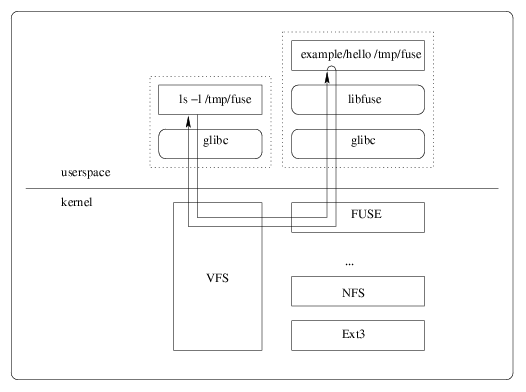
\includegraphics[width=\textwidth]{images/fuse_structure.png}}
\caption{Path of a file system call in the hello world example.}
\label{fig:fuse}
\end{figure}

Figure \ref{fig:fuse} shows the path of a file system call in the provided hello world example file system. We can see the \texttt{FUSE} kernel module acting as a proxy between the \texttt{VFS} system call and the \texttt{example/hello} user space code. A kernel space file system would not need to re-enter user space to compete the system call, hence giving better performance. 

The \texttt{FUSE} library provides a number of function definitions which the user space code implements. These functions are then called when the corresponding file system operation occurs. Some of the important operations are discussed below.

\begin{lstlisting}[language=C, caption={\texttt{FUSE} read operation.}, frame=single]
int read(const char *path, char *buf, size_t size, off_t offset, struct fuse_file_info *fi);
\end{lstlisting}

\noindent
The \texttt{read} function is called when a file system read occurs. It requests that \texttt{size} bytes of the file \texttt{path} starting at offset \texttt{offset} should be written to the buffer \texttt{buf}.

The \texttt{write} function is similar:

\begin{lstlisting}[language=C, caption={\texttt{FUSE} write operation.}, frame=single]
int write(const char *path, const char *buf, size_t size, off_t offset, struct fuse_file_info *fi);
\end{lstlisting}

\noindent
It requests that \texttt{size} bytes from the buffer \texttt{buf} should be written to the file \texttt{path} starting at offset \texttt{offset}.

Similar functions exist for all of the standard file system operations, all of which need to be implemented to provide a fully functional file system.

\subsection{Existing tools}
\label{tools}
The relatively little work on steganography within video was reflected in my search for steganographic programs operating on video files. This section contains an exhaustive list of all the video steganogrphy tools I could find freely\footnote{A further 2 programs exist claiming to embed within video, however these are closed source and not freely available to download. Therefore they have been excluded from this list. (Info Stego, Hiderman)} available on the Internet. A total of 6 tools claimed to provide steganographic embedding functionality within video files. Of these 6, only 3 actually attempt to embed within the video data itself. None of the identified programs allow the user to embed more than one file\footnote{Admittedly you could embed a compressed archive using these tools to effectively allow a directory structure to be embedded.}  and none of them provide any sort of file system interface.

\subsubsection{StegoStick}

\texttt{StegoStick}\textsuperscript{\cite{stegostick}} claims to allow users to ``hide any file into any file''. This statement suggests that the program is simply appending the requested file to the end of the cover object. This suspicion is partly true; based on the file extension, \texttt{StegoStick} splits cover objects into 3 categories: images, media and other. The other category does indeed just append the file to the cover object, whereas the image and media category do attempt to employ steganographic embedding methods. The images category applies to files with extensions \texttt{JPG}, \texttt{GIF} and \texttt{BMP} and uses LSB embedding within \texttt{BMP} files (other image formats are converted to \texttt{BMP} prior to embedding). The media category applies to \texttt{WAV}, \texttt{AVI} and \texttt{MPG} files and assumes each format has a ``header'' of 44+55 bytes\footnote{Listed in the source as ``44 byte header + 54 bytes of extension space''.}. Although this seems to be true for the \texttt{WAV} format, this is not the case for \texttt{AVI} nor \texttt{MPG} files. \texttt{StegoStick} will then use blind LSB embedding within the remaining data. As such, my attempts to use \texttt{StegoStick} to embed within \texttt{AVI} files rendered the resulting video unplayable. % (I haven't actually done this...) 

\subsubsection{StegoMagic}

\texttt{StegoMagic}\textsuperscript{\cite{stegomagic}} claims to ``work on all types of files and all size of data'' which again sounds as though it's appending the file to the end of the cover object. This is indeed the case, embedding an image within a video and inspecting the modified file shows that data has just been appended to the end of the video, albeit encrypted. \texttt{StegoMagic} does not specify the encryption algorithm used and the source code is not available to view. Furthermore, the user cannot specify an encryption key to use. Instead, \texttt{StegoMagic} generates a 5 digit number during the embedding process and echos this to the user.  

\subsubsection{TCSteg}

\texttt{TCSteg}\textsuperscript{\cite{tcsteg}} is a Python script accompanying a blog post written by Martin Fiedler discussing hiding \texttt{TrueCrypt} volumes within \texttt{MP4} files. The method described embeds the \texttt{TrueCrypt} volume within the \texttt{MP4} atom \texttt{mdat} and modifies the chunk offset table within the \texttt{moov} atom so that any application playing the video will ignore the embedded data. A nice property of \texttt{TCSteg} is that the resulting video file can be directly mounted by \texttt{TrueCrypt} since it ignores the \texttt{MP4} header data prior to the embedded volume.\\

\noindent
The above programs all resort to embedding within video files by either appending the embedded data to the end of the video, or inserting the embedded data at some point within the video file. I do not consider this approach to embedding data secure, and it should be a trivial task for any steganalyst to detect the presence of embedded data within the stego objects using a simple hex editor. Therefore, the above stegosystems should be considered broken and definitely not used for the hiding of sensitive data.

\subsubsection{StegoVideo}

\texttt{StegoVideo}\textsuperscript{\cite{stegovideo}} is a Virtual Dub filter\footnote{Which is also available in a stand alone executable form.} which allows users to embedded a file within \texttt{AVI} files (supporting multiple compression codecs). I am unsure of the exact steganograhpic embedding algorithm used since the program is closed source, but the website does mention that \texttt{StegoVideo} makes use of error correction codes to allow embedded data to be recovered even after the resulting video has been compressed - although this is understandably dependant on the compression amount. \texttt{StegoVideo} attempts to protect the embedded data via the use of a passkey (a 5 digit number), although as with \texttt{StegoMagic}, this is not provided by the user and is instead generated and presented to the user to make a note of.

\subsubsection{OpenPuff}

\texttt{OpenPuff}\textsuperscript{\cite{openpuff}} is a steganographic tool supporting a wide range of formats, including \texttt{3GP}, \texttt{MP4}, \texttt{MPG} and \texttt{VOB}. It allows users to embed a file within a collection of carrier objects and uses 3 user provided passwords to encrypt, scramble and whiten (mixing with a high amount of noise) the provided file. Plausible deniability is also provided via the option to add decoy content. \texttt{OpenPuff} successfully embedded and retrieved a text file within a sample \texttt{MP4} video and I could notice no perceivable impact on video quality. Performance was also good due to multithreading support. However, the embedding capacity is very limited. A hard limit of \SI{256}{\mega\byte} is imposed regardless of the number and size of the carrier objects and I was only able to achieve embedding capacities of around 0.0043\%\footnote{2,600 bytes within a \SI{60}{\mega\byte} video.} even at the maximum capacity setting. This makes \texttt{OpenPuff} impractical for hiding large files - for example, you would need around 770 \SI{60}{\mega\byte} \texttt{MP4} carrier files to embed a standard \SI{2}{\mega\byte} \texttt{JPEG} image.

\subsubsection{Steganosaurus}

\texttt{Steganosaurus}\textsuperscript{\cite{steganosaurus}} is a cross platform steganograhpic program developed by James Ridgway. It allows users to embed a file within \texttt{MP4} (\texttt{H264}) video files via the modification of motion vectors. Two embedding algorithm variants are provided and the input file is encrypted using \texttt{AES} with a user provided passphrase. A modified version of \texttt{FFmpeg} was used to access and modify the motion vectors, these modifications have not yet been open sourced. I unfortunately could not get \texttt{Steganosaurus} to run on my computer (using Linux or Windows) and therefore could not test its operation.\\

\noindent
The above 3 programs are much more promising from a steganogrphic security point of view and some of them also support multiple video formats. However, all feature the same limitation of only allowing the user to embed one chosen file and the offered embedding capacities are far from practical for use with large files.

This project aims to remedy these issues by providing the user the opportunity to embed an arbitrary number of files within a video via a file system interface and providing high capacity steganographic embedding algorithms offering capacities in excess of 100\%\footnote{This specifically means a file of size n bytes can have more than n hidden bytes residing inside it.} of the cover object's size\footnote{This is very much a trade off - capacities larger than the file size will come at the sacrifice of steganogrphic security. However, this decision is presented to the user rather than decided by the program itself.}. 

\subsection{Requirements Analysis}

After reviewing the necessary background material and investigating current available solutions to the problem of steganography within video, the following collection of requirements were produced. For the project to be considered a success, at least all of the core requirements should be fulfilled.

\subsubsection{Core Requirements}

\texttt{Stegasis} should:

\begin{enumerate}
\item Allow users to embed data within video files:
	\begin{enumerate}
		\item Several steganographic embedding algorithms should be available.
		\item Each embedding algorithm, $\mathcal{A}$, should satisfy correctness. That is,
		\begin{center}
			$\forall ~\textbf{c}, \textbf{k}, \textbf{m}. ~Ext_{\mathcal{A}}(Emb_{\mathcal{A}}(\textbf{c}, \textbf{k}, \textbf{m}), \textbf{k}) = \textbf{m}$.
		\end{center}
		\item Embedding should occur with no perceivable impact on video quality.
		\item Steganalysis tools should be developed to test the security of the proposed embedding algorithms.
		\item An optional user provided password should encrypt data prior to embedding.
		\item A capacity option should allow users to specify the percentage of each video frame to embed within.
	\end{enumerate}
\item Provide a file system interface:
	\begin{enumerate}
		\item The presented logical volume should reside at a user provided mount point.		
		\item Data written to the file system should be embedded on the fly within the chosen video file.
		\item Data accessed from the file system should be retrieved on the fly from within the video.
		\item Standard file system operations such as creating, deleting and moving files should work as expected, and standard Unix tools such as \texttt{cp}, \texttt{mv} and \texttt{rm} should also work as expected.
	\end{enumerate}	
\item Support raw uncompressed \texttt{AVI} video:
	\begin{enumerate}
		\item Uncompressed \texttt{AVIs} should be natively parsed allowing access to individual pixel data.
	\end{enumerate}	
\item Provide adequate file system performance:
	\begin{enumerate}
		\item Full HD video content should be playable directly from within the presented file system (bitrates of full HD video are roughly 8 - 12 Mb/s\textsuperscript{\cite{bitrate}}).
		\item Ideally, the file system should provide read and write speeds comparable to those provided by USB 2.0 devices\footnote{Although the USB 2.0 standard supports speeds of up to 480 Mb/s, devices rarely reach this theoretical limit.}(roughly 20 MB/s\textsuperscript{\cite{usb2}}).
	\end{enumerate}		
\end{enumerate}

\subsubsection{Possible Extensions}

If time constraints allow, the following extension tasks shall also be completed.\\

\noindent
\texttt{Stegasis} should:

\begin{enumerate}
\item Support a wide range of video formats:
	\begin{enumerate}
		\item Specifically including the popular video format \texttt{MP4}.		
	\end{enumerate}
\item Allow directory operations within the file system:
	\begin{enumerate}
		\item Creating directories using the \texttt{mkdir} command should work as expected, as should using the \texttt{mv} and \texttt{rm} commands.
		\item Organising files within directories should also work as expected.
	\end{enumerate}	
\item Embed also within audio data:
	\begin{enumerate}
		\item Data should also be embedded within the (possible) audio stream of the video, therefore increasing the embedding capacity.
	\end{enumerate}	
\item Provide plausible deniability:
	\begin{enumerate}
		\item A second file system should be (optionally) embedded within the video, mountable with a second passphrase.
		\item The presence of the second, hidden file system should not be detectable.
	\end{enumerate}
\item Be evaluated for perceivable video impact using an evaluation study:
	\begin{enumerate}
		\item A developed web application should evaluate the requirement ``Embedding should occur with no perceivable impact on video quality.'' by obtaining data from multiple users.
	\end{enumerate}		
\end{enumerate}

\subsection{Choice of Languages and Tools}

With the above requirements for the final product defined, an appropriate set of languages and tools can be identified.

It is first noted that \texttt{Stegasis} (as developed for this project) will only function on the \texttt{Linux} operating system. That is, there is no requirement for \texttt{Stegasis} to be cross platform.  

The file system is an important aspect of \texttt{Stegasis} and so it is initially decided which approach to take in developing it as this will influence the later choice of an appropriate programming language. As described within section \ref{fs}, it was decided to use the \texttt{FUSE} library to develop the file system component in user space.

We now address the choice of primary programming language for the development of \texttt{Stegasis}.

Several of the core (and extension) requirements strongly suggest a lower level language such as C or C++ rather than a higher level sandboxed language such as Java. For example, the parsing and modification of \texttt{AVI} files lends itself to a language like C since it will involve large amounts of byte level manipulation. Furthermore, the Microsoft file format reference defines the different data structures used within \texttt{AVIs} as C \texttt{structs}. The identified library for implementing the file system aspect - \texttt{FUSE} - is natively a C library (as is the \texttt{libjpeg} library, and libraries provided by \texttt{FFmpeg}). Although wrappers for other languages (including Java) do exist\textsuperscript{\cite{javafuse} \cite{turbojpeg}}, they seem to be lacking documentation and few are being actively maintained. The requirement that \texttt{Stegasis} should support several steganographic embedding algorithms implores the use of object oriented techniques; defining a \texttt{SteganographicAlgorithm} interface of which each embedding algorithm implements. This suggests C++ over C. The final core requirement, performance, also favours C/C++ over Java\footnote{There have been numerous studies showing that C/C++ code performs better than equivalent Java code\textsuperscript{\cite{javaper1} \cite{javaper2} \cite{javaper3}}.} due to the JVM overheads. 

The reasons above led to the conclusion that C++ should be the primary language used to develop \texttt{Stegasis}.

As discussed in section \ref{ffmpeg}, \texttt{FFmpeg} will be used for the extension task ``\texttt{Stegasis} should support a wide range of video formats'', to allow the decoding and conversion of the many video formats available today, together with library \texttt{libjpeg} discussed in section \ref{jpeg} for the manipulation of \texttt{JPEG} images. 

During the implementation of \texttt{Stegasis}, a number of small steganalysis programs will be developed. These will likely be written in a scripting language such as Python or Matlab since both have extensive library support for mathematical operations.

The extension task ``\texttt{Stegasis} should be evaluated for perceivable video impact using a web application'' will require a website to be developed and hosted for easy access to participants and a database to store the collected user data. \texttt{Node.js} together with the web application framework \texttt{Express} and the database \texttt{MongoDB} was chosen as the development stack for the site. This decision was mainly due to the speed at which you can develop \textit{CRUD} (create, read, update and delete) web applications - essentially what this evaluation site is - and my previous experience with the technologies.


\section{Implementation}

\subsection{Introduction}

The development of \texttt{Stegasis} consisted of the 5 main stages sectioned within this chapter. Firstly, a parser for the \texttt{AVI} file format as discussed in section \ref{avi} was developed allowing direct access to video pixel data. Next, steganographic embedding algorithms were implemented along with corresponding steganalysis tools to test the security of the proposed techniques. The file system was then developed utilising the \texttt{AVI} decoder and steganogrphic algorithms to embed and extract data directly into and out of video files. Finally, the extension tasks were individually addressed providing support for multiple video formats, directory structures and plausible deniability\footnote{The evaluation site extension task is discussed within the evaluation chapter.}. The testing section provides an overview of the testing processes applied throughout development. 

The actual software development process taken differs from that laid out below; each section was not wholly completed before moving onto the next. Instead, an iterative process was taken across all sections, embracing the modern ``Launch early, iterate often'' methodology\textsuperscript{\cite{iterate}}. For example, as specified in the project proposal timetable, a simplified version of \texttt{Stegasis} was initially produced only offering one simple embedding algorithm and basic file system functionality. This allowed integration issues to be identified early on, when the code was still very malleable. Once this basic version was working, an iterative approach was then taken to add more functionality and features. For the sake of readability, I have structured the sections below to group together implementation details for each separate component.

\subsection{AVI Decoder}
\label{avidec}

The concept of an \texttt{AVI} decoder is first abstracted to that of a generic \texttt{Video Decoder} interface\footnote{The term ``interface'' is used as shorthand for an abstract C++ base class. That is, a class with pure virtual member functions and no function implementations.} The core requirements state that the \texttt{AVI} decoder should allow access to individual pixel data. The pixel data within an \texttt{AVI} file is grouped into chunks, one per video frame. It was therefore decided to define the \texttt{Video Decoder} to allow access to the video pixel data at a granularity of a single video frame. It would also be useful for the \texttt{Video Decoder} interface to expose metadata about the video, for example, the total number of video frames in the video, the height and width of the video frames and the total size (in bytes) of each video frame.

This gives the definition for the \texttt{Video Decoder} interface as described in listing \ref{viddec} (\texttt{NextFrameOffset} will be discussed in section \ref{fsi}):

\begin{lstlisting}[language=C++, caption={Video Decoder interface (\texttt{video/video\_decoder.h:15})},frame=single, float,floatplacement=H,label=viddec]
class VideoDecoder {
  public:
    virtual Chunk *getFrame(int frame) = 0;
    virtual int getFileSize() = 0;
    virtual int getNumberOfFrames() = 0;
    virtual int getFrameSize() = 0;
    virtual int getFrameHeight() = 0;
    virtual int getFrameWidth() = 0;
	
    virtual void getNextFrameOffset(int *frame, int *offset) = 0;
    virtual void setNextFrameOffset(int frame, int offset) = 0;
   	   
    virtual void setCapacity(char capacity) = 0;
    virtual void writeBack() = 0;
    virtual ~VideoDecoder() {};
};
\end{lstlisting}

Note that \texttt{getFrame} returns a \texttt{Chunk} wrapper object, rather than a raw \texttt{char} pointer to the frame pixel data, adhering to the \textit{Dependency Inversion} principle\textsuperscript{\cite{inver}}. This will be useful when dealing with different video formats that don't necessarily group all of a frames video data to be accessible by a single \texttt{char} pointer.

A \texttt{Chunk} abstracts the concept of a single frames video data. In the case of uncompressed \texttt{AVI}, this can be thought of as a \texttt{char} pointer to the GBR pixel data, along with an associated frame size in bytes. A boolean value is also associated with each chunk, signifying if the chunk data has been modified, that is, it is dirty.

The \texttt{Chunk} interface is therefore defined as follows:

\begin{lstlisting}[language=C++, caption={Chunk interface (\texttt{video/video\_decoder.h:4})}, frame=single]
class Chunk {
  protected:
    long chunkSize;
  public:
    virtual long getChunkSize() = 0;
    virtual char *getFrameData(int n=0, int c=0) = 0;
   
    virtual bool isDirty() = 0;
    virtual void setDirty() = 0;
};
\end{lstlisting}

\noindent
Note that the parameters for \texttt{getFrameData} are optional. For the \texttt{AVI} decoder, these will not be used.

The \texttt{AVI} parssing process can be thought of consisting of two main parts; parsing the video headers and parsing the video chunk data. The pseudocode in algorithm \ref{parseavi} illustrates this with the headers being parsed lines 1-12 and the chunks being parsed lines 15-22.

\begin{algorithm}[!h]
\caption{\texttt{AVI} parsing process}
\label{parseavi}
\begin{algorithmic}[1]
\State f $\gets$ open(file\_path)
\State riff\_header $\gets$ readRiffHeader(f)
\If{riff\_header.fourCC != RIFF}
	\State print ``File is not an AVI file"
	\State Exit
\EndIf
\State avi\_header $\gets$ readAviHeader(f)
\State bitmap\_info\_header $\gets$ readBitmapInfoHeader(f)
\If{bitmap\_info\_header.compression != 0}
	\State print ``Stegasis does not natively support compressed AVI files''
	\State print ``Rerun using the -f flag''
	\State Exit
\EndIf
\State audio\_info\_header $\gets$ readAudioInfoHeader(f)
\State frame\_chunks $\gets$ [ ]
\State i $\gets$ 0
\Comment{File pointer is now positioned at the start of the audio video chunks} 

\While{i $<$ avi\_header.total\_frames}
	\State chunk $\gets$ readChunk(f)
	\If{chunk.fourCC == 00db}
		\State frame\_chunks[i].chunkSize = chunk.chunkSize
		\State frame\_chunks[i].frameData = readChunkData(f)
		\State i ++
	\Else
		\State Advance f chunk.chunkSize bytes
		\Comment{Chunk was not a video chunk}
	\EndIf
\EndWhile
\end{algorithmic}
\end{algorithm}

See the appendix section B for some longer code samples. The actual implementation is slightly more complex than presented above due to the existence of \texttt{JUNK} chunks. The \texttt{AVI} file format specifies that any number of chunks with a \texttt{FourCC} code of \texttt{JUNK} and of arbitrary length can be inserted between any \texttt{AVI} list structures. The parser must therefore be able to cope with this.

The \texttt{WriteBack} function of the \texttt{AVI} decoder will write back any modified \texttt{Chunk} data into the original \texttt{AVI} file. This operation is described in algorithm \ref{writeback} below.

\begin{algorithm}[!h]
\caption{\texttt{AVI} write back process}
\label{writeback}
\begin{algorithmic}[1]
\State Seek f to the chunks offset
\State i $\gets$ 0
\While{i $<$ avi\_header.total\_frames}
	\State chunk $\gets$ readChunk(f)
	\If{chunk.fourCC == 00db}
		\If{frame\_chunks[i].isDirty}
			\State Write frame\_chunks[i].frameData to f
			\State frame\_chunks[i].dirty = false
			\Comment{This chunk is no longer dirty}
		\Else
			\State Advance f chunk.chunkSize bytes
			\Comment{Chunk did not need to be written}
		\EndIf
		\State i ++
	\Else
		\State Advance f chunk.chunkSize bytes
		\Comment{Chunk was not a video chunk}
	\EndIf
\EndWhile
\end{algorithmic}
\end{algorithm}

The remaining functionality of the parser is mostly trivially returning data from the \texttt{aviHeader} structure (for example \texttt{aviHeader.height}, \texttt{aviHeader.totalFrames} etc.) The only other function of interest is \texttt{getFrameSize}, which returns the number of bytes within each frame that can be embedded within. This (incorrectly) assumes that each frame can always have the same number of bytes embedded within it. This assumption is however true for the steganographic algorithms presented in the next section\footnote{It is also true for the simple \texttt{JPEG} embedding algorithms used within the extension tasks.}, and is implemented as in listing \ref{framesize}.

\begin{lstlisting}[language=C++, caption={\texttt{AVI} decoder \texttt{frameSize} function (\texttt{video/avi\_decoder.cc:298})}, frame=single, label=framesize]
virtual int frameSize() {
  return (int)floor(this->aviHeader.width * this->aviHeader.height * 3 * (capacity / 100.0));
};
\end{lstlisting}

This expression arises from the fact that uncompressed \texttt{AVI} uses 24 bits per pixel value. Since there are $height \cdot width$ pixels within a single frame, multiplying this by 3 will give the total number of bytes. \textit{Capacity} is a user provided percentage ranging in value from 1 - 100. It specifies the percentage of the frame to embed within. \texttt{frameSize} must therefore reduce the returned frame size value by ``capacity percent''.

The effect of the capacity parameter is illustrated within figure \ref{cap50}. 

\begin{figure}[!h]
\centerline{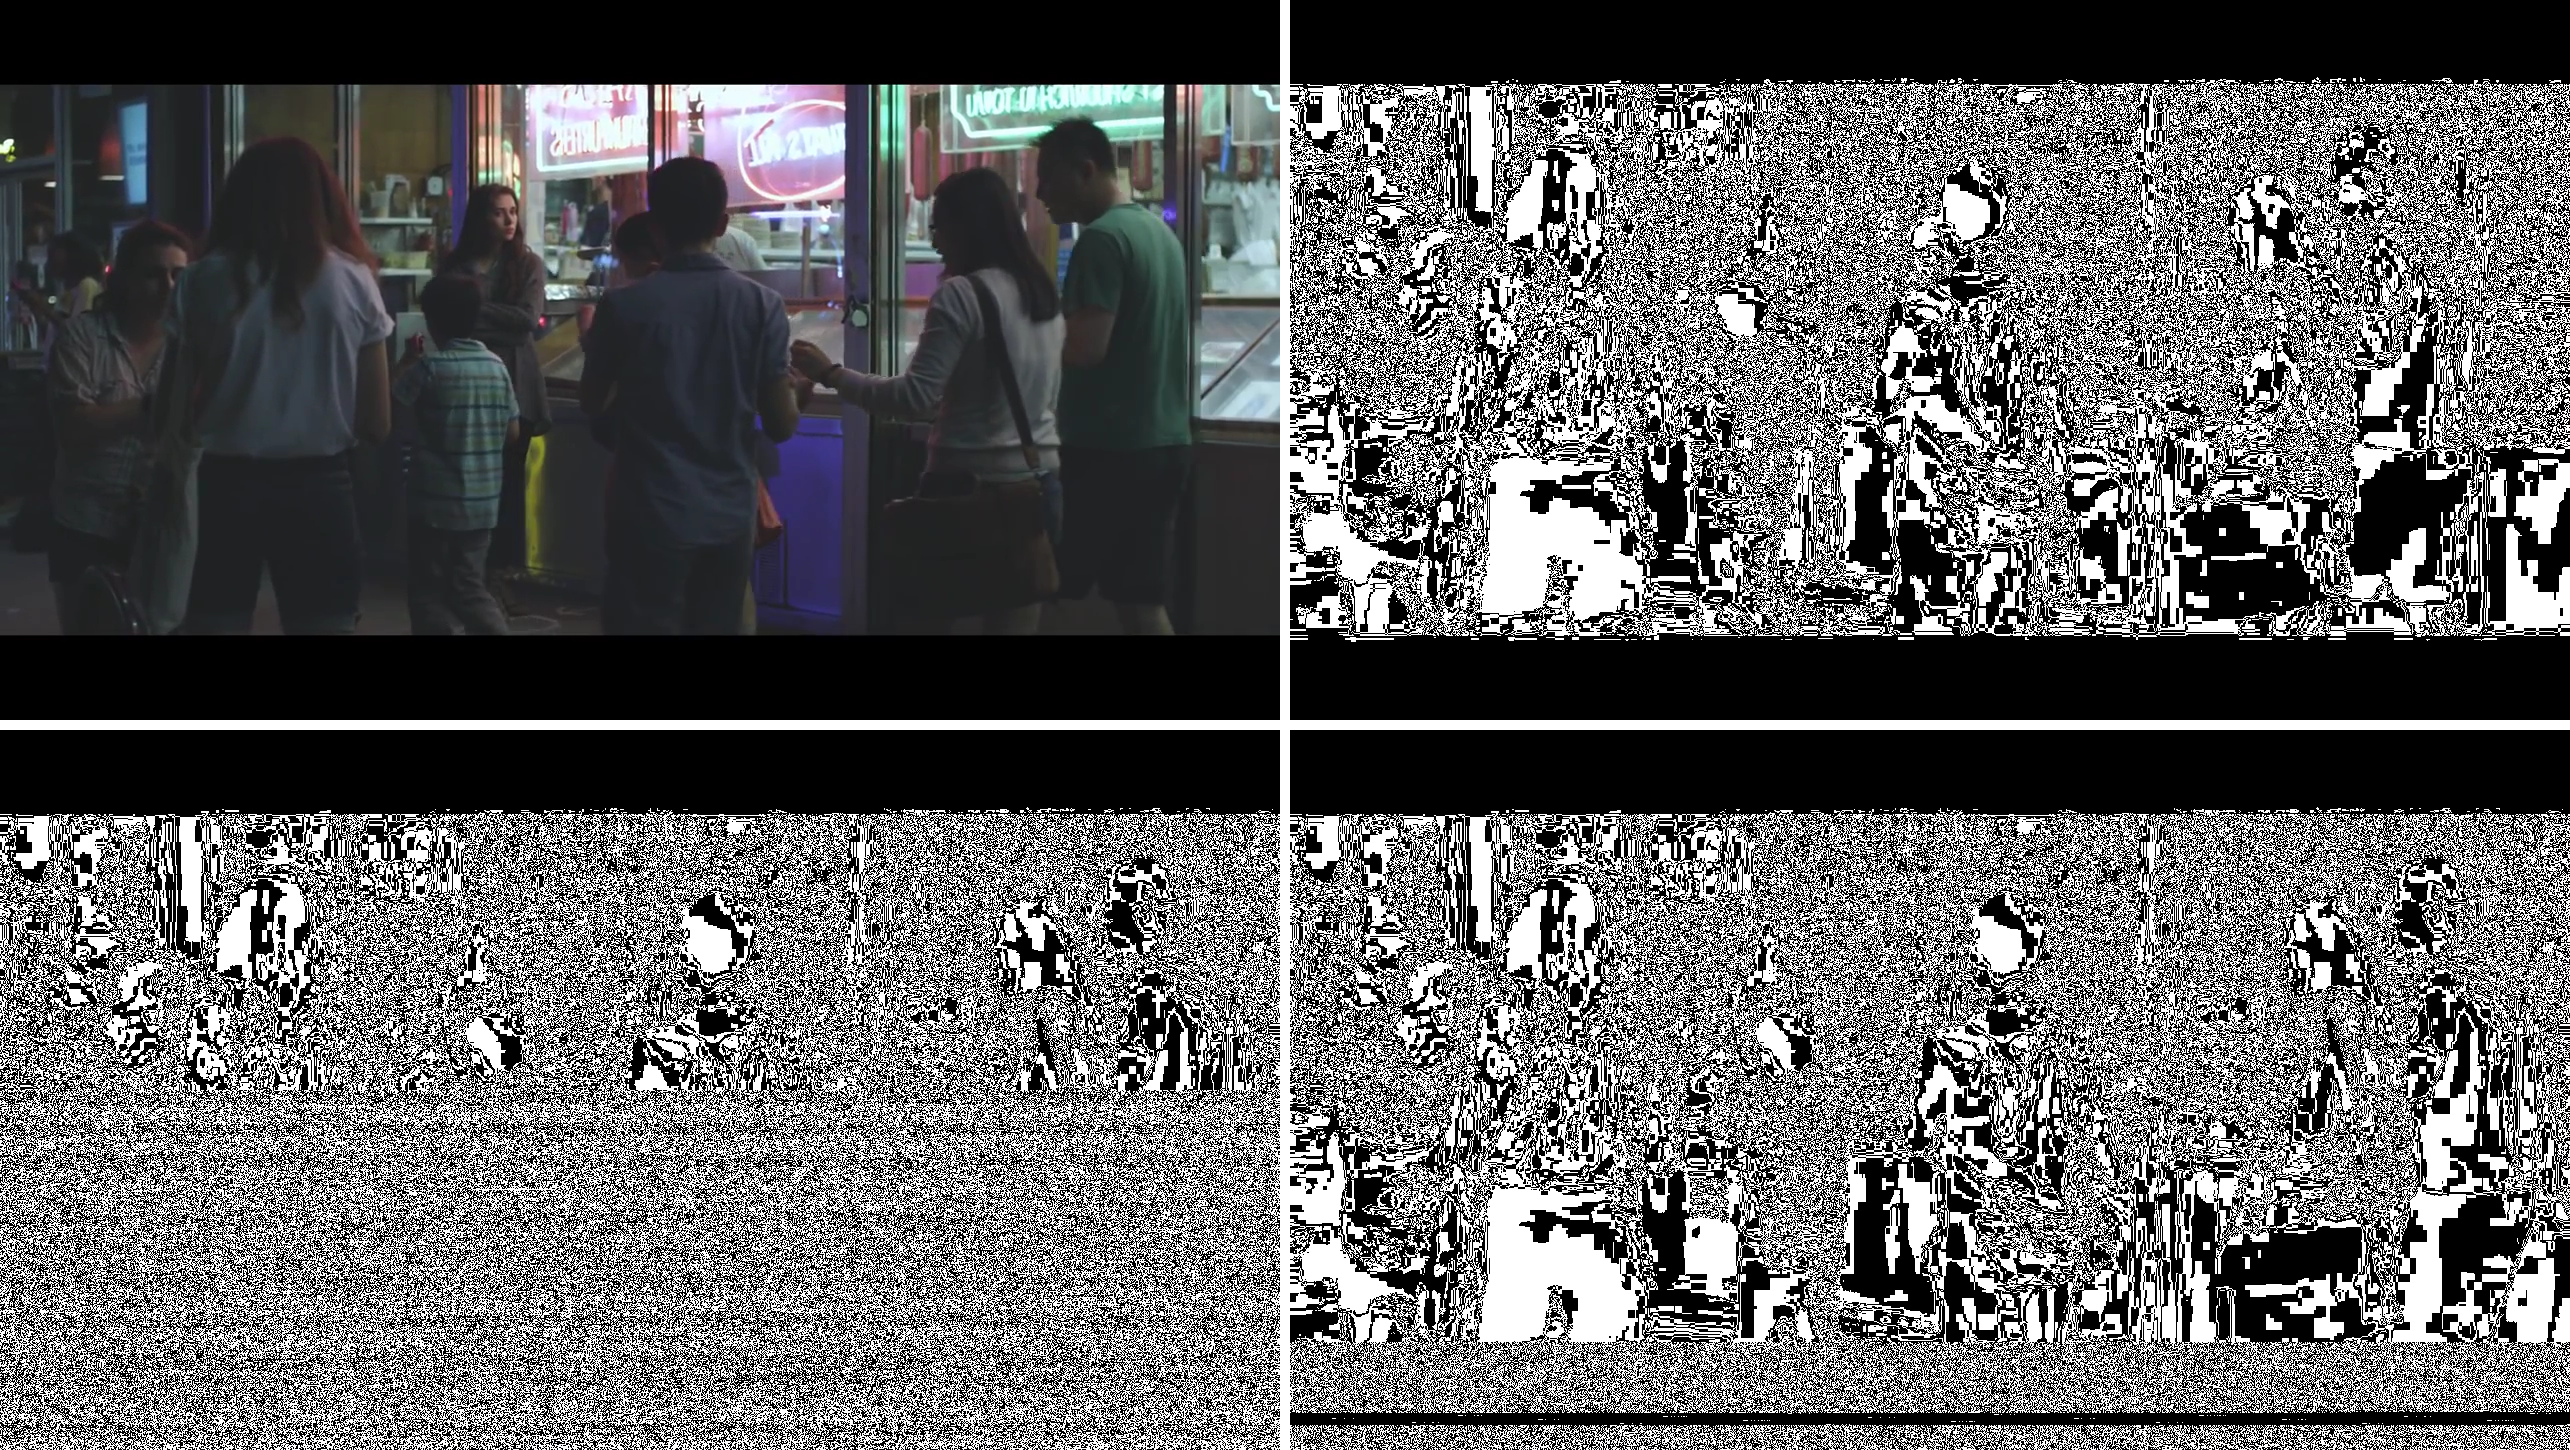
\includegraphics[width=\textwidth]{images/cap_ill.png}}
\caption{Illustration of the capacity parameter.}
\label{cap50}
\end{figure}

\noindent
The top left image is the original video frame and the top right image is the LSB plane (red channel) of the frame with no data embedded. The bottom two images have data sequentially embedded within them using capacity settings of 50\% and 15\% respectively.


The \texttt{AVI} decoder as described now provides all necessary functionality to allow the modification of pixel data to achieve the steganogrphic embedding of information within video frames. 


\subsection{Steganographic Algorithms}

The concept of a generic stegangraphic embedding algorithm is initially developed and implemented as a \texttt{Steganographic Algorithm} interface. As defined within the background discussion of steganogrphic concepts, a steganogrphic system consists of a pair of functions providing embedding and extraction functionality. The interface will therefore need to declare two functions \texttt{embed} and \texttt{extract} which will embed and extract data respectively. The \texttt{Video Decoder} interface defined above allows access to video data via individual frame \texttt{Chunk} objects. It was therefore decided to define the \texttt{embed} and \texttt{extract} functions to operate on \texttt{Chunk} objects. Listing \ref{stegoalg} shows the final interface.

\begin{lstlisting}[language=C++, caption={\texttt{Stego Algorithm} interface (\texttt{steg/steganographic\_algorithm.h:8})}, frame=single, label=stegoalg]
class SteganographicAlgorithm {
  protected:
    string password;
    VideoDecoder *dec;
  public:
    virtual void embed(Chunk *c,char *data,int dataBytes,int offset)=0;
    virtual void extract(Chunk *c,char *output,int dataBytes,int offset)=0;
    virtual void getAlgorithmCode(char out[4]) = 0;
};
\end{lstlisting}

\noindent
The \texttt{embed} function should be read as ``embed \texttt{dataBytes} bytes from \texttt{data} into chunk \texttt{c} starting at an offset \texttt{offset} bytes into the frame''. Similarly, the \texttt{extract} function should be read as ``extract \texttt{dataBytes} bytes from chunk \texttt{c} starting at an offset \texttt{offset} bytes into the frame and put them into \texttt{output}''. It was decided to place the error handling logic within the file system code. The steganogrphic algorithm implementations therefore do not contain any such logic and instead assumes that the pointer \texttt{data} does indeed point to at least \texttt{dataBytes} bytes and so on.

\texttt{getAlgorithmCode} simply returns a (unique) 4 character algorithm identifier which is used when users specify which algorithm they want to use.\\

\noindent
Implementations of the \texttt{Steganographic Algorithm} interface are now presented along with corresponding steganalysis methods. 

\subsubsection{LSB Sequential Embedding}

Sequential LSB embedding is arguably the simplest steganographic algorithm. It works by replacing the LSBs of the cover object with the bits comprising the message, producing the stego image. Algorithm \ref{lsbalg} shows pseudocode for the LSB embedding algorithm. The matching extraction algorithm is shown in algorithm \ref{lsbext}.


\begin{algorithm}[!h]
\caption{LSB embedding algorithm}
\label{lsbalg}
\begin{algorithmic}[1]
\For{i $\gets$ 0 upto dataBytes - 1}
	\For{j $\gets$ 7 downto 0}
		\If{The jth significant bit of data[i] == 1}
			\State Set LSB(frame[offset++]) to 1
		\Else
			\State Set LSB(frame[offset++]) to 0
		\EndIf
	\EndFor
\EndFor
\end{algorithmic}
\end{algorithm}

\begin{algorithm}[!htb]
\caption{LSB extraction algorithm}
\label{lsbext}
\begin{algorithmic}[1]
\For{i $\gets$ 0 upto dataBytes - 1}
	\For{j $\gets$ 7 downto 0}
		\State Set the jth significant bit of output[i] to LSB(frame[frameByte++]) 
	\EndFor
\EndFor
\end{algorithmic}
\end{algorithm}

\noindent
The actual implementation is relatively short and so is included below in listing \ref{lsbimp}.

\begin{lstlisting}[language=C++, caption={LSB implementation (\texttt{steg/lsb\_algorithm.cc:8})}, frame=single, label=lsbimp]
virtual void embed(Chunk *c, char *data, int dataBytes, int offset) {
  char *frame = c->getFrameData();
  for (int i = 0; i < dataBytes; i ++) {
    for (int j = 7; j >= 0; j --) {
      if ((((1 << j) & data[i]) >> j) == 1) {
        frame[offset++] |= 1;
      } else {
        frame[offset++] &= ~1;
      }
    }
  }
};
\end{lstlisting}

\noindent
The operation of the sequential LSB embedding algorithm is illustrated in figure \ref{lsbill}.

\begin{figure}[!htb]
\centerline{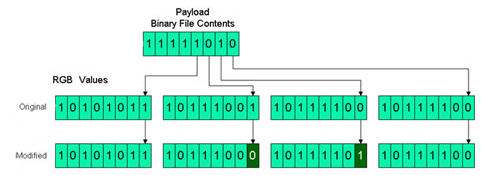
\includegraphics[width=\textwidth]{images/lsb_ill.png}}
\caption{Illustration of the LSB Embedding algorithm.}
\label{lsbill}
\end{figure}

Using the algorithm as shown above, \SI{43.2}{\kilo\byte} of data is is embedded into a 1280 $\times$ 720 resolution video frame (a capacity setting of 100\%). The result of this is shown in figure \ref{lsbemb_full}. The left image is the cover object and the right image is the stego object. 

\begin{figure}[!h]
\centerline{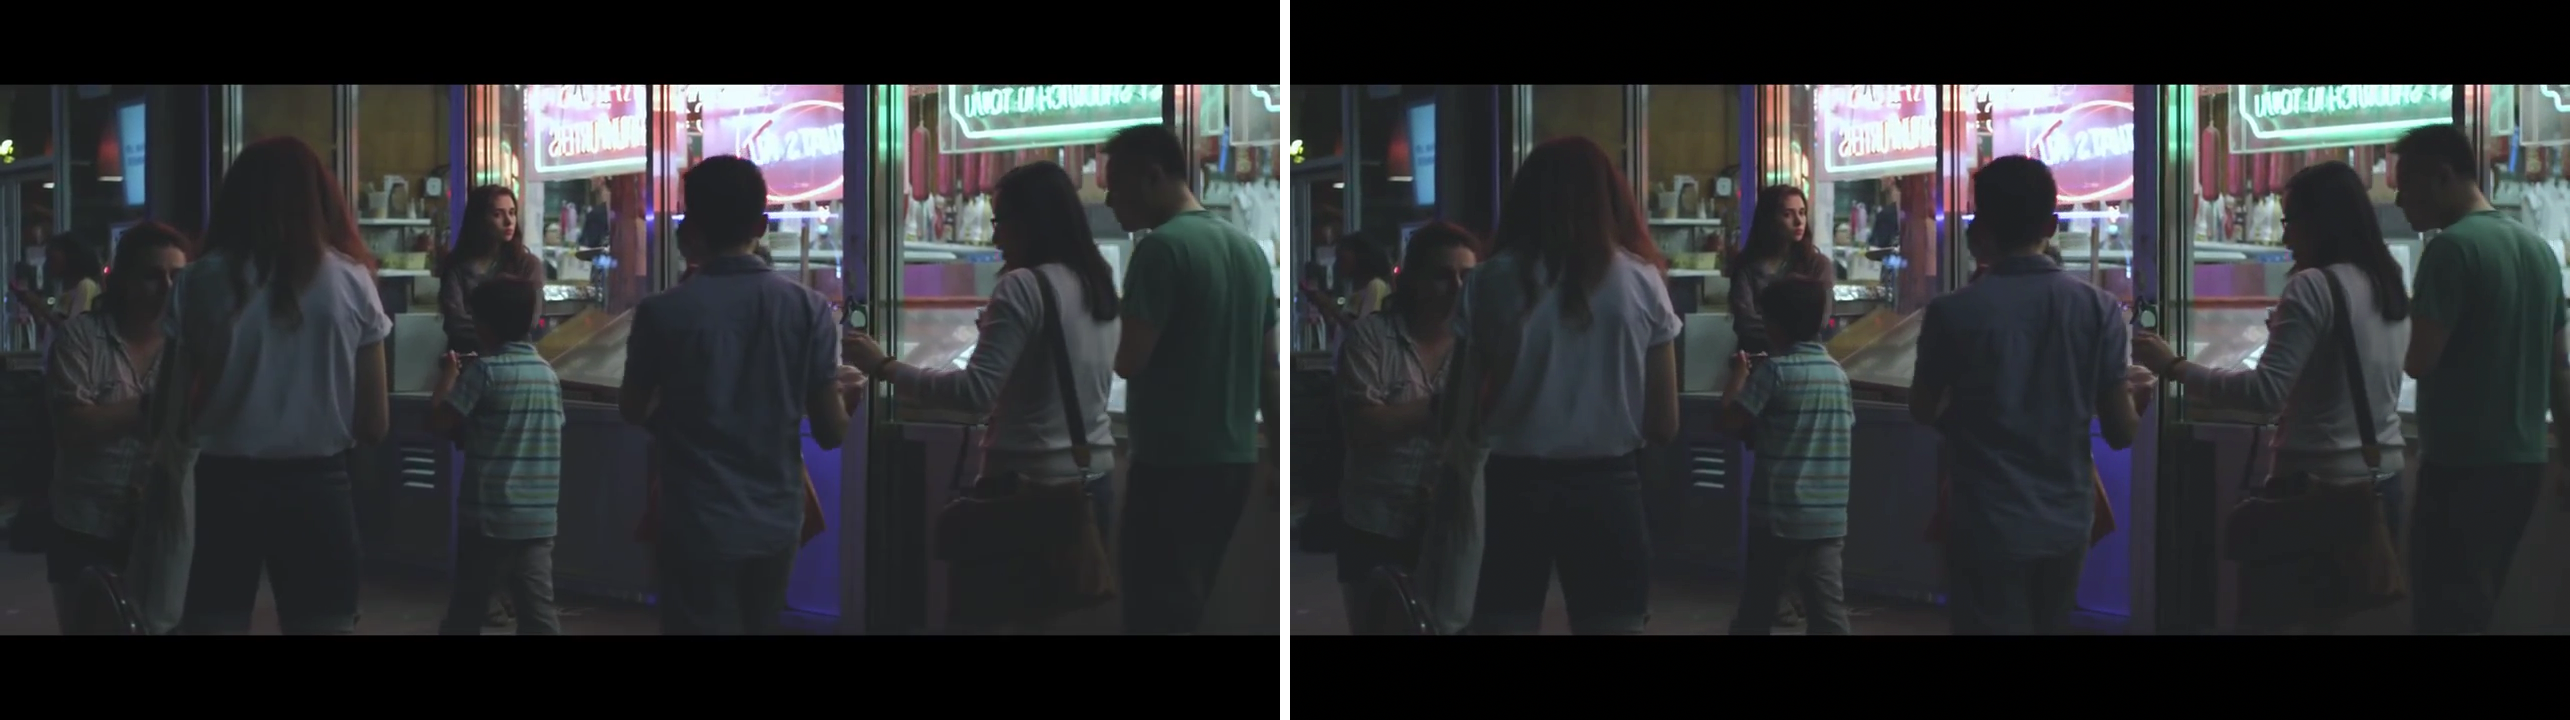
\includegraphics[width=\textwidth]{images/lsb_emb_full.png}}
\caption{Effect of the LSB Embedding algorithm.}
\label{lsbemb_full}
\end{figure}

\noindent
The visual impact on the video frame is very small and almost certainly not noticeable having been reproduced within this document at a smaller resolution. However, if we take a closer look at a specific portion of the video frame, we can see some small discrepancies between the cover and stego objects - see figure \ref{lsbcloseup}. I am unsure how well these images will be reproduced when printed, but the difference is definitely noticeable within the \texttt{PDF}. Note that without the original cover object for comparison, it would be very hard (if not impossible) to identify these details visually and deduce the presence of embedded data. However, if the LSB plane of the frame is visually inspected, as in figure \ref{lsbemb}, one can immediately detect the presence of the hidden data - the LSB plane of the stego object looks ``too random''. This is an example of a \textit{visual steganalysis attack}.


\begin{figure}
\centerline{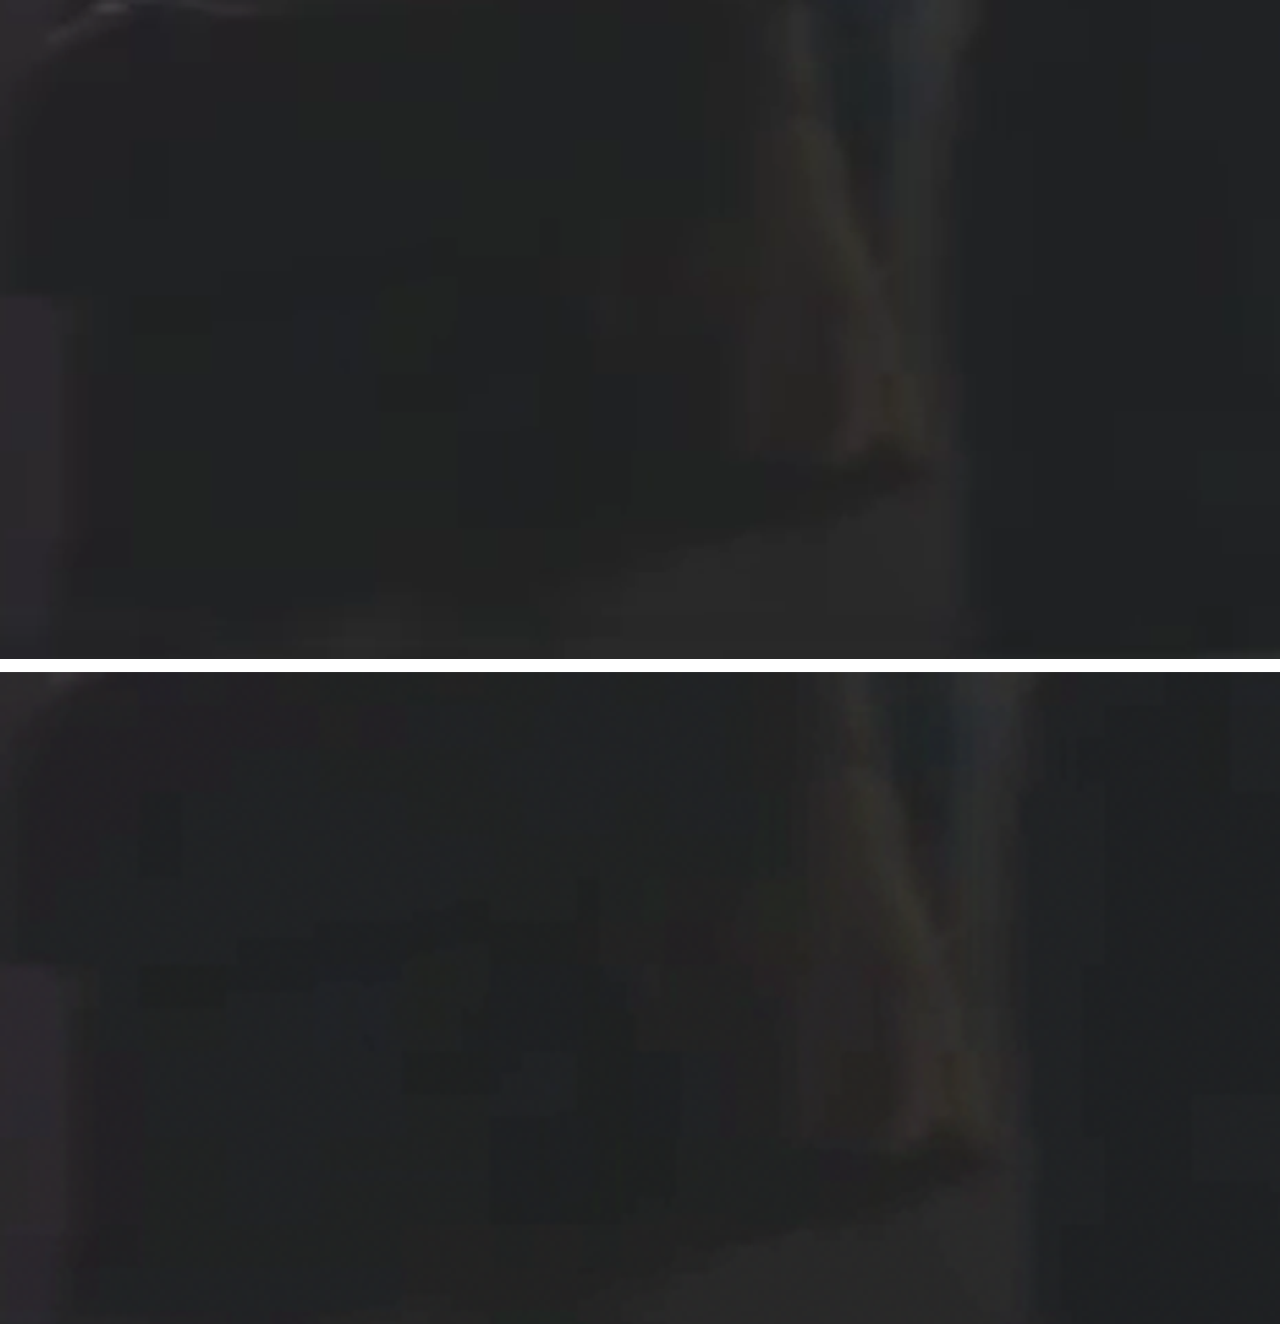
\includegraphics[width=0.9\textwidth]{images/closeup_3.png}}
\caption{Close up effect of the LSB Embedding algorithm.}
\label{lsbcloseup}
\end{figure}


\begin{figure}
\centerline{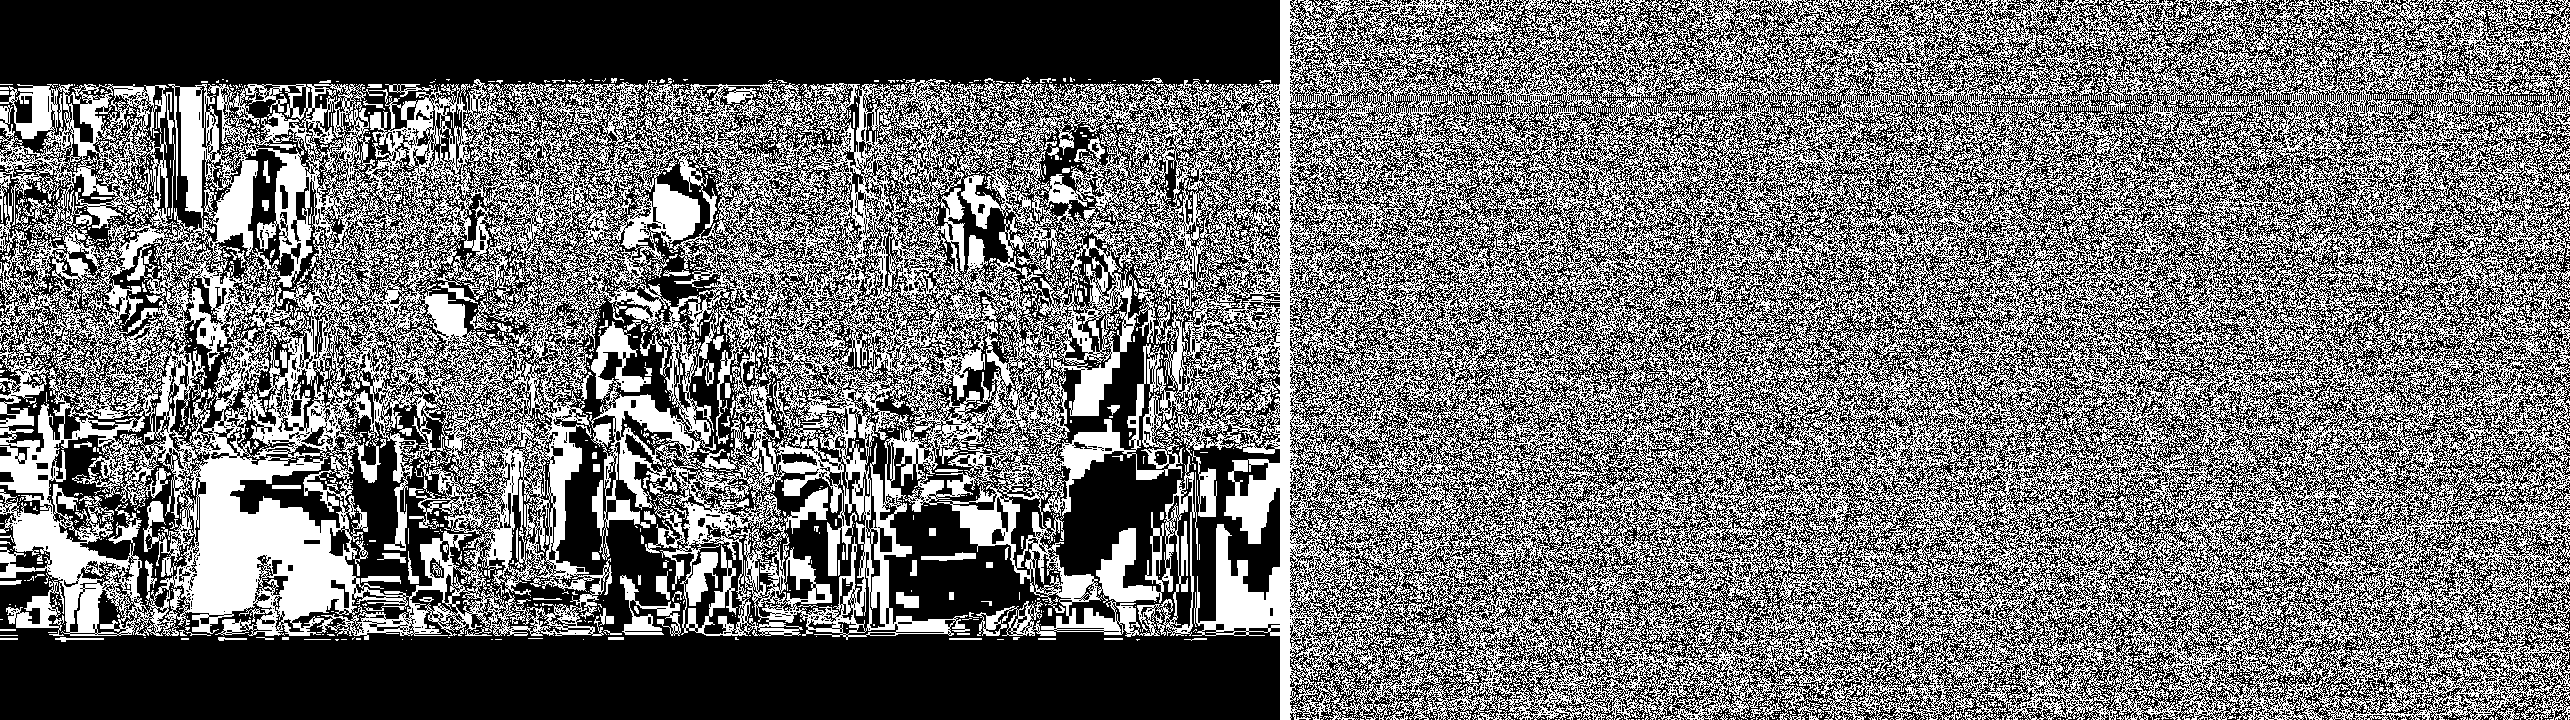
\includegraphics[width=0.9\textwidth]{images/lsb_emb.png}}
\caption{LSB plane of the cover and stego object.}
\label{lsbemb}
\end{figure}

Formalising the looking ``too random'' idea leads to another steganalysis attack known as the \textit{Chi-Squared attack} developed by Westfeld and Pfitzmann\textsuperscript{\cite{chi}}. To implement the Chi-Squared attack, the concept of \textit{Pair of Values} (PoVs) is first introduced.

One of the results of an embedding algorithm like sequential LSB embedding is the creation of POVs, pixel values that embed into one another. For example, a pixel value of 100 in the cover image will either stay 100 or change to 101. Similarly, a pixel value of 101 will either stay 101 or change to 100. Thus (100, 101) is a POV. 

\begin{ddef}
\textsc{Pairs of Values}\\[5pt]
A POV $\textbf{p}$ is a member of the set $\mathcal{P}ov$, defined as,
\begin{center}
$\mathcal{P}ov \triangleq \{~(2k, 2k + 1) ~\vert ~ 0 \leq k \leq 127 ~\}$
\end{center}
\end{ddef}

\noindent
Westfeld and Pfitzmann claim that the LSBs in images are not completely random, rather, the frequencies of each of the two pixel values in each POV tend to lie far from the mean of the POV. That is, it is unlikely for the frequency of pixel value $2k$ to be close to equal to the frequency of pixel value $2k+1$. Furthermore, as information is embedded into the cover object, the frequencies of $2k$ and $2k+1$ become (nearly) equal. The Chi-squared attack was designed to detect this and bases the probability of embedding on how close to equal POVs are in the image.

To implement the attack, the following steps are taken in reference to a given image. First, $x_{k} =$ frequency($2k$) and $y_{k} =$ frequency($2k+1$) are calculated, followed by the expected frequency $z_{k} = \dfrac{x_{k} + y_{k}}{2}$ $~\forall ~k$. $n$ is defined to be the number of POVs, $\vert \mathcal{P}ov \vert$. For uncompressed \texttt{AVI} using 24 bits per pixel, $n=128$. The \textit{minimum frequency condition} is now applied. This sets $x_{k} = y_{k} = z_{k} = 0$ and decrements $n$ by one, if the condition $x_{k} + y_{k} \leq 4$ holds. The Chi-Squared statistic, with $n - 1$ degrees of freedom is then calculated:
\begin{center}
$\chi ^{2} _{n-1} = \mathlarger{\sum}\limits_{k=0}^{127} \dfrac{(x_{k} - z_{k})^2}{z_{k}}$
\end{center}

\noindent
The probability of embedding, $p$, is then calculated by evaluation of the following integral:
\begin{center}
$p = 1 - \dfrac{1}{2^{\frac{n-1}{2}} \Gamma (\frac{n-1}{2})} \mathlarger{\int}_{0}^{\chi ^{2} _{n-1}} e^{-\frac{u}{2}}u^{\frac{n-1}{2}-1} du$
\end{center}

\noindent
See appendix section \ref{app:chi} for an implementation of the Chi-squared attack in Python.\\

\noindent
The Chi-squared attack produces very good results for the na\"ive sequential LSB embedding algorithm. Figure \ref{chi} show an example of it in use operating on a video frame with a capacity setting of 50\%. It obvious that information has been embedded within the firth half of the frame.\\

\begin{figure}[here]
\centerline{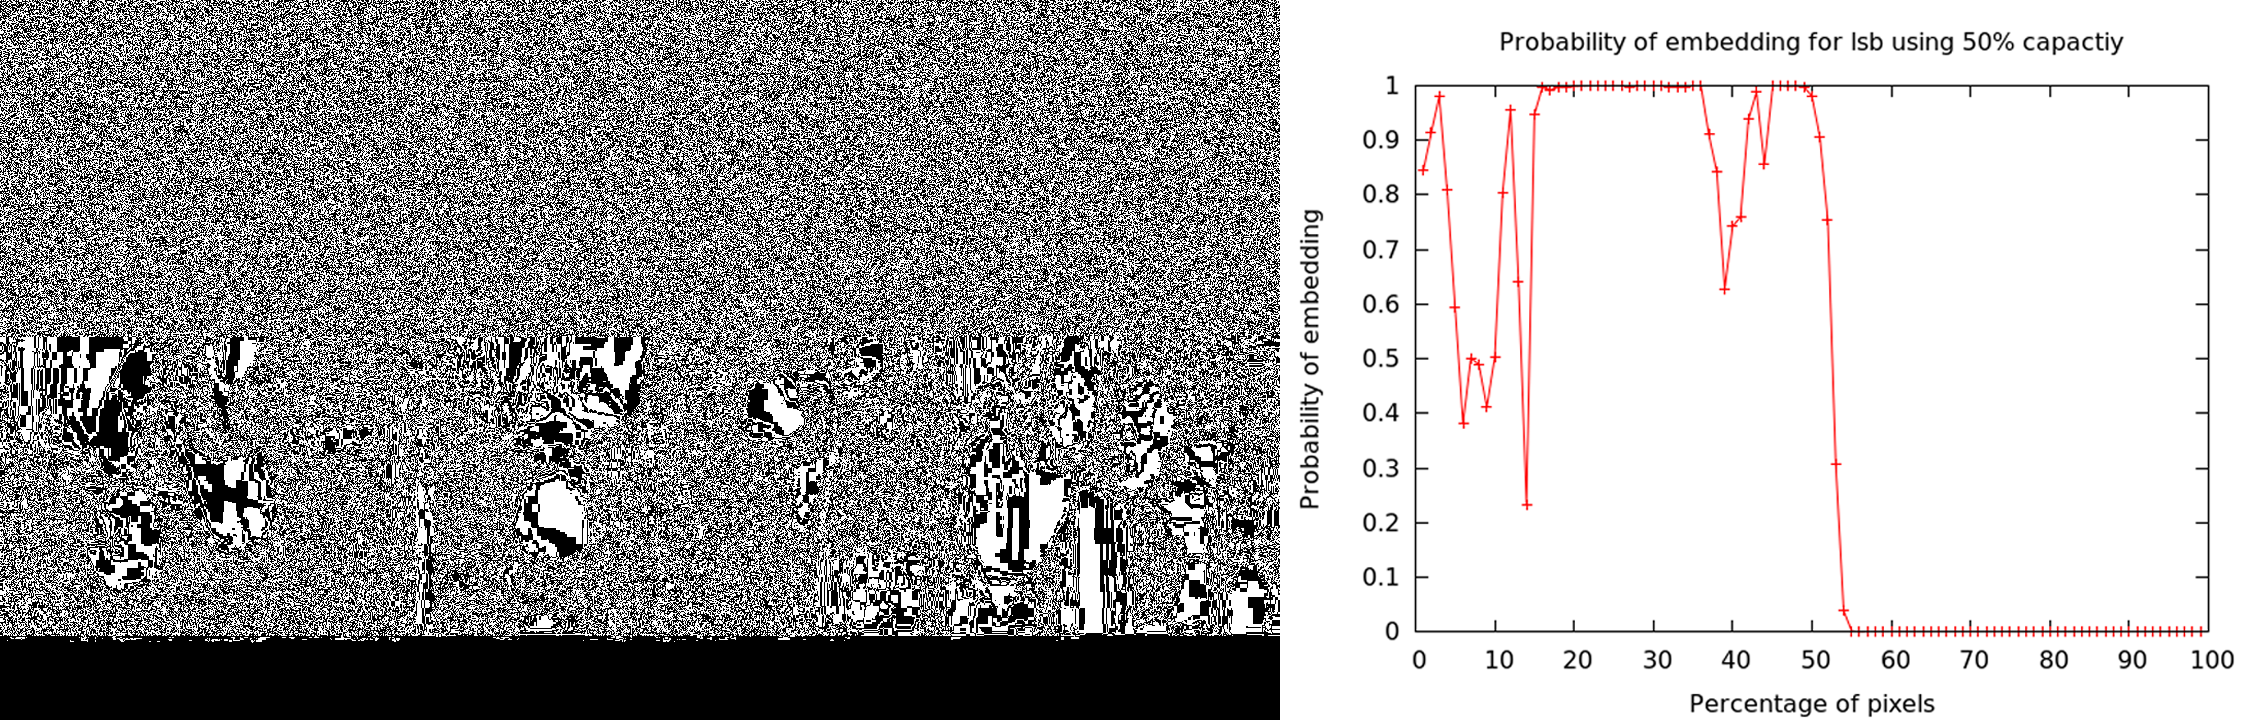
\includegraphics[width=\textwidth]{images/chi_graph.png}}
\caption{Results of the Chi-Squared attack.}
\label{chi}
\end{figure}

\noindent
The Chi-Squared attack motivates the development of a \textit{permuted} LSB embedding algorithm. The attack works so well because regardless of the capacity setting, the data is sequentially embedded from the top of the video frame. It would be better to distribute the data uniformly throughout the entire frame. A permuted LSB embedding algorithm achieves this and resists the Chi-Squared attack when using a small capacity setting.\footnote{Of course, a permuted embedding using a capacity of 100\% is comparatively no different to sequential embedding!}.

\subsubsection{Permuted LSB Embedding}

One can produce deceptively simple pseudocode for the permuted LSB embedding algorithm as shown in algorithm \ref{lsbp}.

\begin{algorithm}[!h]
\caption{Permuted LSB embedding algorithm}
\label{lsbp}
\begin{algorithmic}[1]
\State path $\gets$ a pseudorandom permutation of the cover object
\State path.seekToOffset(offset-1)
\For{i $\gets$ 0 upto dataBytes - 1}
	\For{j $\gets$ 7 downto 0}
		\If{The jth significat bit of data[i] == 1}
			\State Set LSB(frame[path.next()]) to 1
		\Else
			\State Set LSB(frame[path.next()]) to 0
		\EndIf
	\EndFor
\EndFor
\end{algorithmic}
\end{algorithm}

\noindent
Lines 1 and 2 hide a large amount of complexity involved in actually implementing the permuted LSB algorithm.

Assuming the cover object consists of $n$ bytes, a pseudorandom permutation of the cover object can be thought of as a pseudorandom permutation of the numbers 0 - $n$. The obvious way to produce a pseudorandom permutation of a list of numbers is to shuffle an array containing them. This approach has the drawback that you need to hold the numbers in memory (\SI{11}{\mega\byte} for a single 720p HD video frame). Instead, a different approach using a \textit{Linear Congruential Generator}\textsuperscript{\cite{lcg}} (LCG) was taken.

\begin{ddef}
\textsc{Linear Congruential Generator}\\[5pt]
A Linear Congruential Generator is defined by the recurrence relation:
\begin{center}
$X_{n+1} = (aX_{n} + c) \mod m$
\end{center}
where $X$ is the sequence of pseudorandom values, and
\begin{center}
$m, ~0 < m$ - the modulus\\
$a, ~0 < a < m$ - the multiplier\\
$c, ~0 \leq c < m$ - the increment\\
$X_{0}, ~0 \leq X_{0} < m$ - the seed
\end{center}
are integer constants that specify the generator.
\end{ddef}

\noindent
The Hull-Dobell Theorem\textsuperscript{\cite{hull}} states that a LCG will have a full period if and only if the following 3 requirements are satisfied:
\begin{enumerate}
	\item $gcd(c, m) = 1$ ($c$ and $m$ are relatively prime),
	\item $a-1$ is divisible by all prime factors of $m$,
	\item $a-1$ is a multiple of 4 if $m$ is a multiple of 4.
\end{enumerate}

\noindent
Therefore, if the above requirements can be satisfied, a LCG can be used as a pseudorandom permutation for the cover object with $m$ equal to $n$ (the size of the cover object). Note that forcing $m$ to be a power of 2, simplifies the above requirements to:
\begin{enumerate}
	\item $gcd(c, m) = 1$,
	\item $a-1$ is odd,
	\item $a-1$ is a multiple of 4 if $m$ is a multiple of 4.
\end{enumerate}

\noindent
As such, $m$ is set equal to the next power of 2 larger or equal to $n$. Any produced values larger or equal to $n$ are just thrown away, therefore producing a full period of size $n$ as required.

The pseudorandom permutation should be dependant on a user provided passphrase. Therefore, the values of $a$ and $c$ are determined using a key derived from the users password. The popular key derivation function \texttt{PBKDF2}\textsuperscript{\cite{keyd}} is used along with the \texttt{Whirlpool}\textsuperscript{\cite{pool}} hash function to generate a 128 byte key and the first 4 bytes are taken as an unsigned integer and used to derive $c$ and $a$. Rather than implement these well known algorithms myself, I used the popular C++ cryptographic library, \texttt{Crypto++}.\\

\noindent
This successfully describes an implementation for line 1 of algorithm \ref{lsbp}. Line 2 unfortunately causes some problems for the LCG due to precisely the reason that it was chosen to be used.

Since the full array of the pseudorandom permutation is not being stored, the LCG does not facilitate direct random access. For example, if the 50th element of the permutation is requested, the 49 elements before it must first be calculated starting from $X_{0}$. This had a huge impact on the performance of the algorithm to the point of the file system becoming unusable. Therefore, it was decided to pre-compute a hashmap mapping from frame offsets to the corresponding pseudorandom permutation element, therefore eliminating the need to calculate all elements prior to the requested one. This fixes the performance problems, but now means the entire permutation is being stored in memory - exactly why the original method was rejected! It was decided to remain using the LCG method with only a single global permutation used across all video frames.

The result of the permuted embedding algorithm is illustrated in figure \ref{lsbp_ill}. The left image has data embedded using the sequential embedding algorithm whereas the right image has the same data embedded using the permuted embedding algorithm. Both images were using a capacity setting of 15\%.

\begin{figure}[here]
\centerline{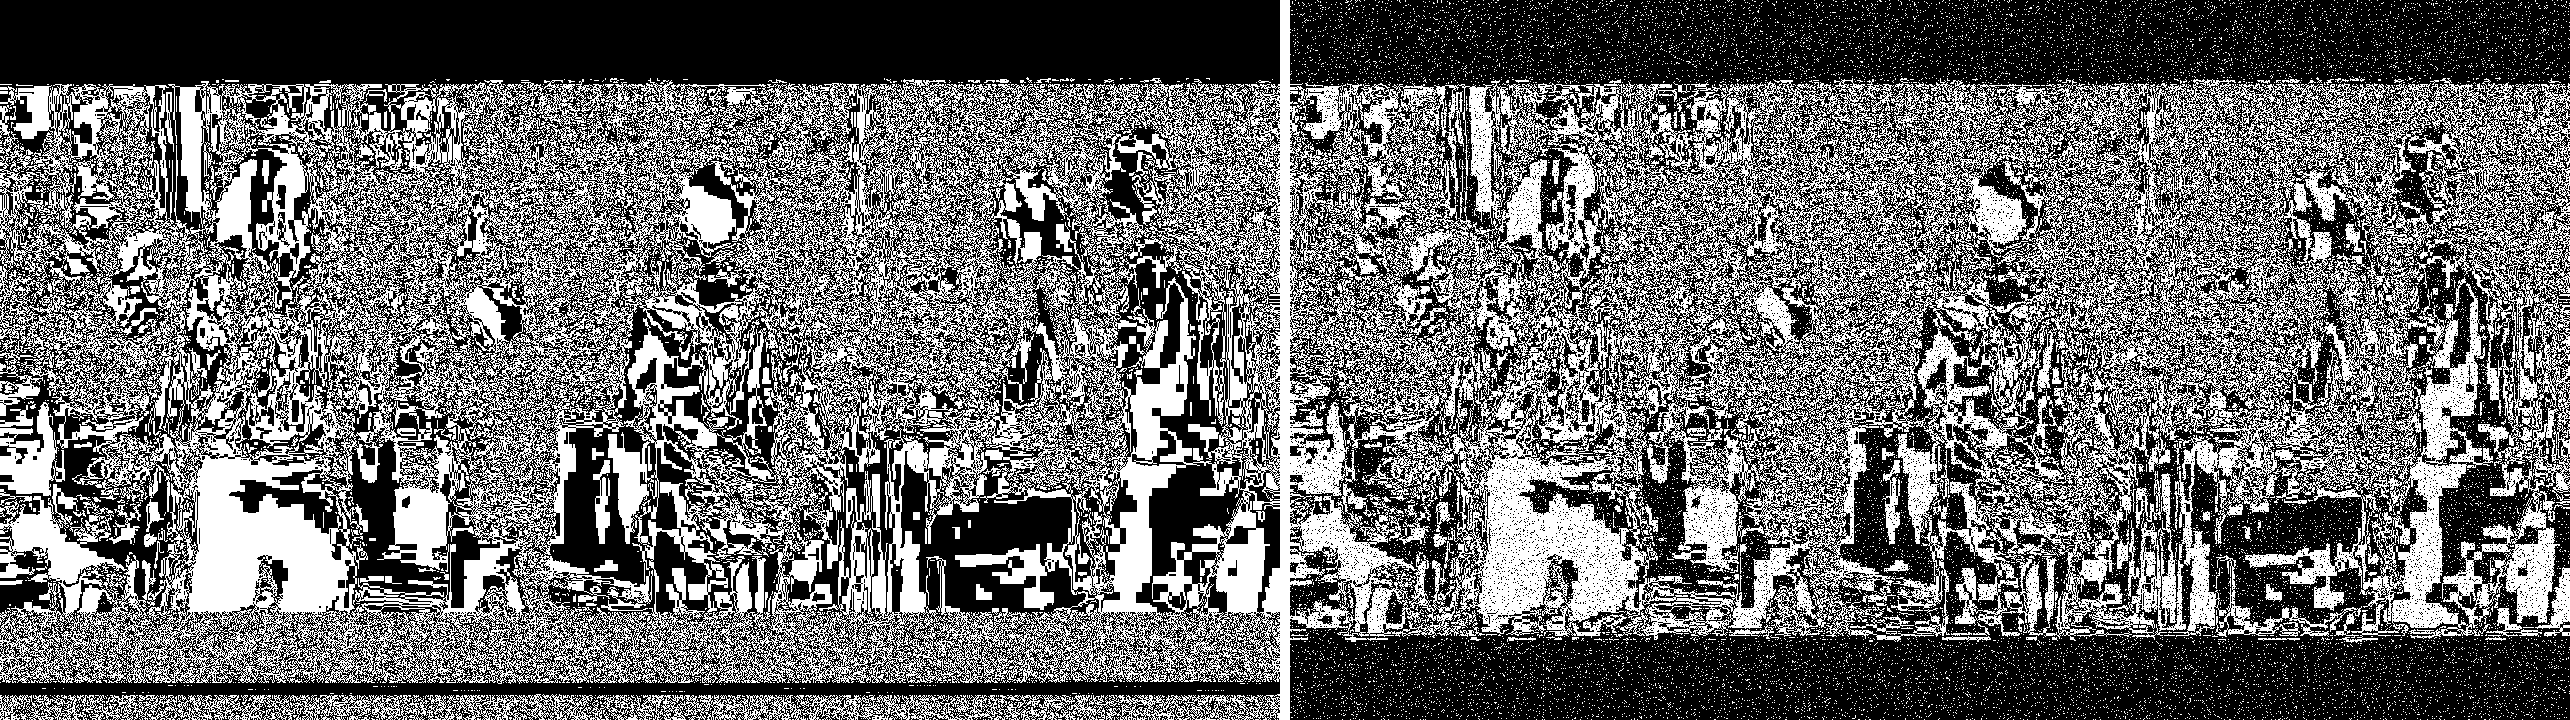
\includegraphics[width=\textwidth]{images/lsbp_ill.png}}
\caption{Illustration of the permuted LSB algorithm.}
\label{lsbp_ill}
\end{figure}

Figure \ref{lsbp_chi} shows the result of applying the Chi-Squared attack to the video frames in figure \ref{lsbp_ill}. The left and right graphs show the probability of embedding within the left and right frame respectively. It is clear that the implemented permuted LSB embedding algorithm resists the Chi-Squared attack when using small values for the capacity setting. 

\begin{figure}[here]
\centerline{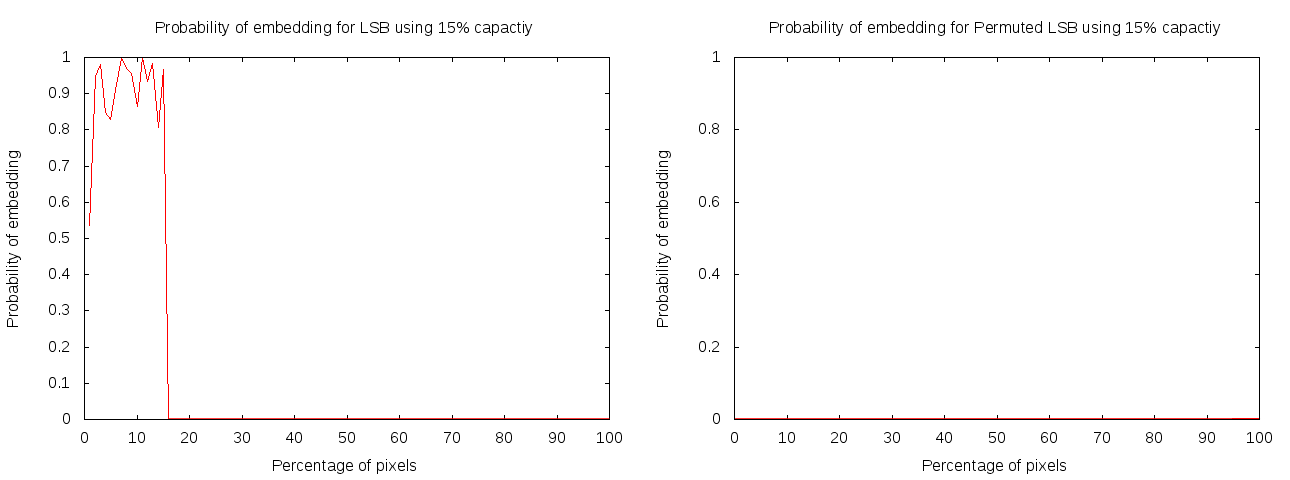
\includegraphics[width=\textwidth]{images/lsbp_chi.png}}
\caption{Chi-Squared attack on the permuted LSB algorithm.}
\label{lsbp_chi}
\end{figure}

\noindent
The above example embedded data within an uncompressed \texttt{AVI} video file which was 10 seconds in duration, had a resolution of $1280\times720$ and was \SI{741}{\mega\byte} in size. Using the permuted LSB embedding algorithm with a capacity setting of 15\% (which resisted the Chi-Squared attack), \texttt{Stegasis} informed me that the formatted volume had a total capacity of \SI{14.49}{\mega\byte}, roughly 2\% of the file size. This embedding capacity is already a lot better than some of the those provided by programs investigated in section \ref{tools}, and will be further improved upon during the extension task within section \ref{extffmpeg}.

\subsubsection{Permuted and Encrypted LSB Embedding}

To further strengthen the security of \texttt{Stegasis}, it was decided to encrypt the data before embedding it within the video. This way, even if the stegosystem is broken, that is the hidden data has been identified and extracted, the information itself will not be compromised. The same user provided passphrase used to permute the data throughout the video frame is used within the encryption process, addressing another concern of some of the investigated programs in section \ref{tools}.\\

\noindent
The initial approach to encrypting the embedded data was to simply \texttt{XOR} it with a pseudorandom number stream. The \texttt{Crypto++} library provided a variety of suitable pseudorandom number generators which could be seeded. It was chosen to use the \texttt{RandomPool} algorithm and to seed it using both the entire 128 byte derived key, and the requested embed offset into the video frame. This way, if the same file is written twice to the volume, it will be encrypted to 2 different byte streams\footnote{Unless the file is embedded within 2 different frames at the same offset.}. Unfortunately, this will cause some problems when the file system is developed in section \ref{fsi}.

Listing \ref{lsb2} shows the implementation of the permuted and encrypted LSB embedding algorithm.

\begin{lstlisting}[language=C++, caption={Encrypted and permuted embedding (\texttt{steg/lsb2\_algorithm.cc:41})}, frame=single, label=lsb2]
virtual void embed(Chunk *c, char *data, int dataBytes, int offset) {
  char *frame = c->getFrameData();
  CryptoPP::RandomPool pool;
  pool.IncorporateEntropy((const unsigned char *)this->key, 128);
  pool.IncorporateEntropy((const unsigned char *)&offset, 4);
  
  int frameByte = lcg.map[offset++];
  for (int i = 0; i < dataBytes; i ++) {
    char xord = data[i] ^ pool.GenerateByte();
    for (int j = 7; j >= 0; j --) {
      if ((((1 << j) & xord) >> j) == 1) {
        frame[frameByte] |= 1;
      } else {
        frame[frameByte] &= ~1;
      }
      frameByte = lcg.map[offset++];
    }
  }
};
\end{lstlisting}

\noindent
More standard encryption algorithms were then added, such as \texttt{AES} (256 bit), \texttt{TwoFish} and \texttt{Serpent}. All of these algorithms are available within the \texttt{Crypto++} library which made incorporating them easy. \texttt{Stegasis} currently supports standard \texttt{AES}, and also \texttt{AES} $\rightarrow$ \texttt{TwoFish} $\rightarrow$ \texttt{Serpent}. That is, the data is first encrypted using \texttt{AES}, the result of this is then encrypted with \texttt{TwoFish} and then \texttt{Serpent}. This method has the advantage that if even 2 of the above algorithms are cryptographically broken, the data will still be secure\footnote{This encryption option is also offered by \texttt{TrueCrypt}.}. You do however incur a performance penalty due to the encryption. This is discussed in detail within the evaluation section \ref{perf}.\\

\noindent
This concludes the steganogrphic embedding algorithms developed to satisfy the core requirements operating on uncompressed \texttt{AVI} video. Although I have shown resistance to some steganalysis techniques, I have no doubt that there exist attacks that would break the implemented stego systems. However, steganogrphic security was not the sole focus of this project and the framework \texttt{Stegasis} provides would allow easy incorporation of new, more secure embedding algorithms.


\subsection{The File system}
\label{fsi}

It was decided early on (and stated within the project proposal) that the file system would only support a subset of the features offered by a fully-fledged standard file system. The following features were considered essential for a practical file system and were planned to be implemented: Creating and deleting files, reading and writing to files, listing the files in the file system and renaming (moving) files. The lack of directory functionality means that all embedded files will reside in the root of the file system. Also note the lack of permissions support, all files will be given the same permissions of \texttt{755} (\texttt{RWXRW-RW-}). Changing a file's access and modification times is also not implemented meaning all times default to 0 \textit{Unix Time} (1 January 1970). Omitting these features does have an impact on the usability of the file system, for example the \texttt{make} command makes use of file modification dates to determine if they need recompiling. However, the file system is not being designed for general purpose use, it is merely supposed to be a container for a collection of files\footnote{However, I would argue that after the directory structure extension task has been implemented, the file system provides enough functionality for most general use cases.}.

Since the file system functionality was being implemented from scratch, the code written turned out complex and intricate due to the many corner cases encountered during integration testing. A large amount of time was dedicated to testing the implemented file system and tracking down particularly nasty concurrency bugs arising in specific circumstances.\\

The basic idea behind storing the file system within a video is to develop some kind of header which contains the locations of all of the files stored across the video frames. The files themselves will be broken into arbitrary sized \textit{chunks} and stored within a particular frame at a particular offset. Consider the following example use case which motivates the solution developed in this section. A 10 byte text file is first written to the volume and embedded within frame 1 of the video at offset 0. A second file is now written to the volume and is such embedded within frame 1 at offset 80\footnote{Since it takes 8 bytes of frame to embed 1 byte of data.}. Now, additional text is appended to the first file, where should this be embedded? The obvious answer is after the second file, thus requiring some sort of header to keep track of the chunks so that the files can be read back correctly.

\subsubsection{Developing the header}

The header serves a similar purpose to the \textit{File Allocation Table} used with the \texttt{FAT} file systems. It will need to be stored in a known location so that it can be extracted when the video file is mounted. It was decided to use the first frame of the video to store the header and is such named the \textit{File Allocation Frame} or \texttt{FAF} for short. The design of the header went through a number of iterations before arriving at the final version presented here, mainly due to underestimating the number of bits needed to store the file frame numbers and offsets. Figure \ref{header} shows the overall structure of the header.

\begin{figure}[!h]
\centerline{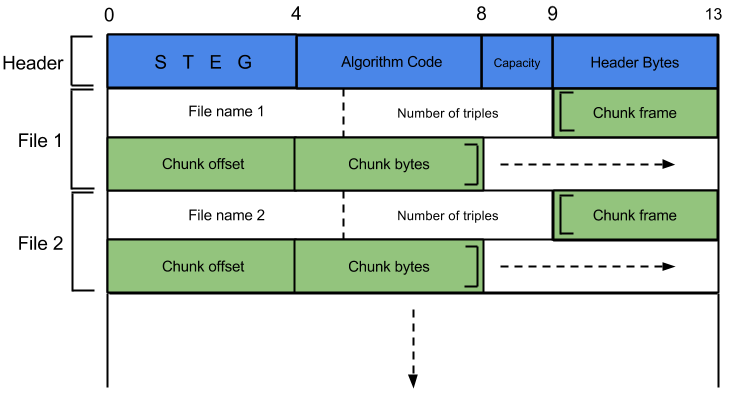
\includegraphics[width=\textwidth]{images/header.png}}
\caption{Header structure overview.}
\label{header}
\end{figure}

\noindent
The header section (coloured blue) contains metadata about the embedded file system. ``STEG'' is the literal 4 character \texttt{ASCII} string and is used to check the header has been correctly extracted. If STEG is not found as the first 4 bytes of the header, the extraction process is aborted and an error message displayed to the user. The ``Header Bytes'' field contains the number of remaining bytes in the header (that is, the size of the header not including the blue coloured section), allowing the extraction of the remaining header data from the \texttt{FAF}. This data contains information for each of the files within the file system, including the file name as a null terminated string, the number of chunks the file is split into and the location and size of each of these chunks. A file chunk is represented as a \texttt{Triple} defined in listing \ref{triple}.

\begin{lstlisting}[caption={Triple definition (\texttt{fs/stegfs.h:19})}, frame=single, label=triple]
struct Triple {
  uint32_t frame;
  uint32_t offset;
  uint32_t bytes;
};
\end{lstlisting}

\noindent
Within figure \ref{header}, a single triple is indicated with square brackets, and is coloured green. A file can contain an arbitrary number of triples each of which can span multiple frames, but note that using an unsigned integer for the struct fields limits individual chunk sizes to (roughly) \SI{4}{\giga\byte}. Also note that only a single frame is used as the \texttt{FAF} - it cannot span multiple frames. This limits the total size of the header, imposing a maximum number of files and chunks.

\subsubsection{Reading and writing the header}

Internally, the header data will be stored in memory as a pair of \texttt{unordered\_maps}, one mapping from file name to file size and the other from file name to a vector\footnote{This is an ordered data structure, the triple contained in vector[0] will contain the file data immediately preceding vector[1].} of \texttt{Triples}. These are named \texttt{fileSizes} and \texttt{fileIndex}.

The process of reading the header is split up into 2 main sections, reading the header data and reading the file data. These are both illustrated within Algorithm \ref{readheader}.

The video decoder get and set frame offset methods, briefly mentioned in section \ref{avidec}, are used to indicate where new files written to this existing file system should be embedded within the video. The read header process identifies the highest frame and offset and passes this data to the video decoder.

Writing back the header is a similar process explained within algorithm \ref{writeheader}.

\begin{algorithm}
\caption{Reading the file system header.}
\label{readheader}
\begin{algorithmic}[1]
\State header\_frame $\gets$ first video frame
\State header\_sig $\gets$ extract 4 characters from header\_frame
\If{header\_sig != STEG}
	\State print ``Video has not been formatted, or invalid password provided.''
	\State Exit
\EndIf
\State algorithm\_code $\gets$ extract 4 characters from header\_frame
\State capacity $\gets$ extract byte from header\_frame
\State header\_bytes $\gets$ extract integer from header\_frame
\While{extracted $<$ header\_bytes}
	\State file\_name $\gets$ extract string from header\_frame
	\State number\_triples $\gets$ extract integer from header\_frame
	\State file\_size $\gets$ 0	
	\For{j $\gets$ 0 upto number\_triples - 1}
		\State triple $\gets$ extract triple from header\_frame
		\State fileIndex[file\_name].append(triple)
		\State file\_size += triple.bytes
	\EndFor
	\State fileSizes[file\_name] $\gets$ file\_size
\EndWhile
\State max\_frame $\gets$ largest frame containing data
\State max\_offset $\gets$ smallest offset within max\_frame data is not embedded within
\State video\_decoder.setNextFrameOffset(max\_frame, max\_offset)
\end{algorithmic}
\end{algorithm}

\begin{algorithm}
\caption{Writing the file system header.}
\label{writeheader}
\begin{algorithmic}[1]
\State header\_frame $\gets$ the first video frame
\State header $\gets$ byte array
\State header\_bytes $\gets$ 0
\State offset $\gets$ 0
\For{(file\_name, triples) in fileIndex}
	\State header[offset] $\gets$ file\_name
	\State offset += file\_name.length() + 1
	\Comment{Null terminated}
	\State num\_triples $\gets$ triples.length()
	\State header[offset] $\gets$ num\_triples
	\State offset += 4
	\For{triple in triples}
		\State header[offset] $\gets$ triple
		\State offset += sizeof(triple)
	\EndFor
	\State header\_bytes += file\_name.length() + 1
	\State header\_bytes += 4
	\State header\_bytes += sizeof(triple)*num\_triples
\EndFor
\State embed header\_bytes into header\_frame
\State embed header into header\_frame
\end{algorithmic}
\end{algorithm}

\subsubsection{Compacting the header}

During testing, it was noticed that writes to the file system seemed to occur in chunks of \texttt{4096} bytes. Due to the above presented design of the file system header, this resulted in relatively large files containing a very large number of chunks, too large to fit into the singe \texttt{FAF}. For example, a \SI{5}{\mega\byte} music file would be written into 1221 chunks. Since each chunk consists of 12 bytes (three 4 byte integers), you would need \SI{14.65}{\kilo\byte} to just store all of the triples into the header. Unfortunately, this meant the largest file you could embedded within any 720p uncompressed \texttt{AVI} (regardless of the length) was \SI{117}{\mega\byte}. This was decided to be an unacceptable limitation and so a process to compact the header and remove unnecessary chunks was developed. Figure \ref{compact} shows a visual representation of this process occurring, green and red lines indicate the start and end of a chunk respectively. The first process compacts sequential chunks of the same file within frames to give single chunks per frame, sequential single frame chunks are then combined in the second process. This allows a file spread across the entire video to be represented by a single chunk.

\begin{figure}[!h]
\centerline{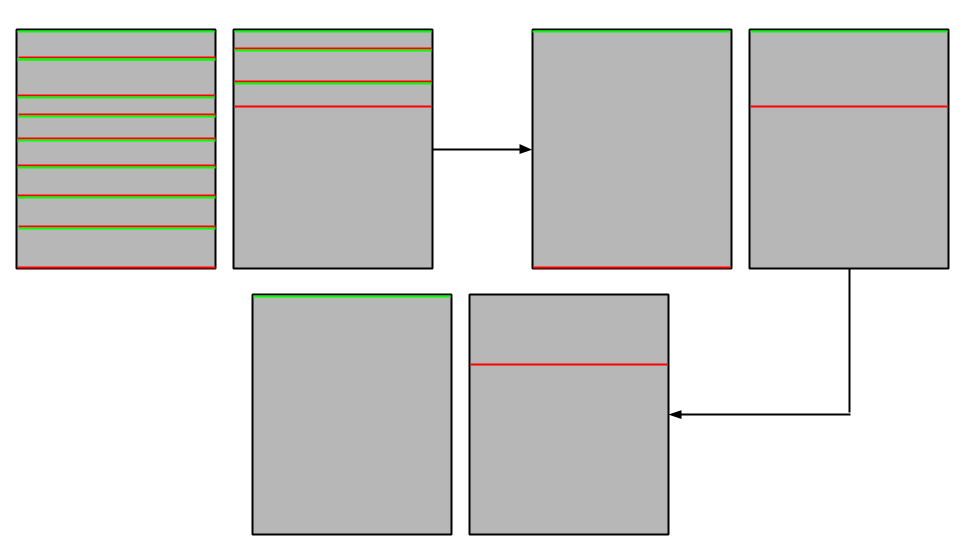
\includegraphics[width=\textwidth]{images/compact.png}}
\caption{Header compaction process.}
\label{compact}
\end{figure}

\subsubsection{Writing to the file system}

A write to the file system will occur in three main stages. First, \texttt{create} will be called requesting that a new file be created with a specified name. Next, the \texttt{write} function will be called a number of times requesting that data be written to the file. Finally \texttt{flush} will be called for the file requesting that any data held in memory be flushed to disk.

The first stage is easy to implement and is listed in listing \ref{create}.

\begin{lstlisting}[language=C++, caption={The \texttt{create} function call (\texttt{fs/stegfs.cc:202}).}, frame=single, label=create,float,floatplacement=!Ht]
int SteganographicFileSystem::create(const char *path, mode_t mode, struct fuse_file_info *fi) {
  this->fileSizes[path] = 0;
  this->fileIndex[path] = std::vector<struct Triple>();
  return 0;
};
\end{lstlisting}

\noindent
The write calls are a bit trickier, recall the \texttt{FUSE} write call which requests that \texttt{size} bytes from the buffer \texttt{buf} should be written to the file \texttt{path} starting at offset \texttt{offset}. Algorithm \ref{write} shows pseudocode for the write function.\\

\begin{algorithm}[!h]
\caption{Writing to the file system.}
\label{write}
\begin{algorithmic}[1]
\State bytes\_written $\gets$ 0
\While{bytes\_written $<$ size}
	\State (next\_frame, next\_offset) $\gets$ decoder.getNextFrameOffset()
	\State frame $\gets$ getFrame(next\_frame)
	\State triple $\gets$ Triple()
	\State triple.frame $\gets$ next\_frame
	\State triple.offset $\gets$ next\_offset
	\State bytes\_left\_in\_frame $\gets$ Frame Size - next\_offset
	\If{size - bytes\_written $<$ bytes\_left\_in\_frame}
		\State		
		\Comment{This frame will finish off this write call}
		\State triple.bytes $\gets$ size - bytes\_written
		\State embed triple.bytes from buf+bytes\_written into frame at offset next\_offset
		\State decoder.setNextFrameOffset(nextFrame, next\_offset + size-bytes\_written)
		\State bytes\_written += size-bytes\_written
	\Else
		\State		
		\Comment{Write all bytes left in frame and go around again}
		\State triple.bytes $\gets$ bytes\_left\_in\_frame / 8
		\State embed triple.bytes from buf+bytes\_written into frame at offset next\_offset
		\State decoder.setNextFrameOffset(nextFrame + 1, 0)
		\State bytes\_written += bytes\_left\_in\_frame / 8
	\EndIf
	\State fileIndex[path].append(triple)
\EndWhile
\State return size
\end{algorithmic}
\end{algorithm}

The above explanation doesn't address the case where writes occur to a file already existent within the file system, that is, it is being overwritten or extended. This is more complicated since it is beneficial to reuse the previously allocated chunks for the file and is therefore listed in the appendix section \ref{app:codewrite}.

Finally, \texttt{flush} is called which will write the header and ask the video decoder to write back to disk. Note the conditional flag \textit{performance}, running \texttt{Stegasis} with the \texttt{-p} flag will cause this process be skipped.

\begin{lstlisting}[language=C, caption={\texttt{FUSE} flush implementation (\texttt{fs/stegfs.cc:537}).}, frame=single,float,floatplacement=!Htb]
int SteganographicFileSystem::flush(const char *path, struct fuse_file_info *fi) {
  if (!this->performance) {
    this->writeHeader();
    this->decoder->writeBack();
  }
  return 0;
};
\end{lstlisting}

\subsubsection{Reading from the file system}

The read function call is similar, recall the declaration which requests that \texttt{size} bytes of the file \texttt{path} starting at offset \texttt{offset} should be written to the buffer \texttt{buf}. The read function must identify the chunk \texttt{offset} points to and then return the correct amount of data possibly spread across multiple subsequent chunks. Algorithm \ref{read} describes the function operation. Note that two cases are needed when extracting data from chunks due to the possibility of data being encrypted. If \texttt{read} requests data from the middle of a chunk, the entire chunk is first decrypted, and then the correct data returned from this.

\begin{algorithm}[!htb]
\caption{Reading from the file system.}
\label{read}
\begin{algorithmic}[1]
\State bytes\_written $\gets$ 0
\State (triple, chunk\_offset) $\gets$ findTriple(offset)
\While{bytes\_written $<$ size}
	\State bytes\_left\_in\_chunk $\gets$ triple.bytes - chunk\_offset
	\State frame $\gets$ getFrame(triple.frame)
	\If{size - bytes\_written $<$ bytes\_left\_in\_chunk}
		\If{chunk\_offset == 0}
			\State extract size-bytes\_written bytes from frame at offet triple.offset into buf+bytes\_written
		\Else
			\State extract entire triple from frame into temp
			\State copy size-bytes\_written bytes from temp+chunk\_offset into buf+bytes\_written 
		\EndIf
		\State return size
	\EndIf
	\If{chunk\_offset == 0}
		\State extract bytes\_left\_in\_chunk bytes from frame at offet triple.offset into buf+bytes\_written
	\Else
		\State extract entire triple from frame into temp
		\State copy bytes\_left\_in\_chunk from temp+chunk\_offset into buf+bytes\_written 
	\EndIf
	\State bytes\_written += bytes\_left\_in\_chunk
	\State chunk\_offset $\gets$ 0
	\State triple $\gets$ getNextTriple()
\EndWhile
\end{algorithmic}
\end{algorithm}

The described algorithm doesn't work for chunks spanning multiple frames as it is rather verbose to list here, a complete version which does is listed in appendix section \ref{app:coderead}.

\subsubsection{Listing files in the file system}

The function \texttt{readdir} is called when the contents of a directory are requested to be listed, the implementation is straightforward and just iterates of the fileSizes map as shown in listing \ref{readdir}.\\

\begin{lstlisting}[language=C++, caption={\texttt{FUSE} readdir implementation (\texttt{fs/stegfs.cc:264}).}, frame=single, label=readdir,upquote=true,float,floatplacement=!Hhbt]
int SteganographicFileSystem::readdir(const char *path, void *buf, fuse_fill_dir_t filler, off_t offset, struct fuse_file_info *fi) {
  filler(buf, '.', NULL, 0);
  filler(buf, '..', NULL, 0);
  for (auto kv : this->fileSizes) {
    filler(buf, kv.first.c_str() + 1, NULL, 0);
  }
  return 0;
};
\end{lstlisting}

\noindent
The above \texttt{FUSE} operations cover the majority of the core file system implementation, successfully implementing all of the decided essential features listed at the start of this subsection.

\subsection{Command line application}

To complete \texttt{Stegasis}, the implemented components must be assembled together and a user interface produced. It was decided that a command line application would be developed allowing the user to utilise the functionality developed within this project. Listing \ref{stegasisrun} shows the process of formatting and mounting a video using \texttt{Stegasis}.

\begin{lstlisting}[caption={Using \texttt{Stagasis} to format and mount a video.}, frame=single, label=stegasisrun]
$ stegasis format -alg=lsbp -pass=password -cap=25 ~/my_video.avi
Formatting video...
Volume size: 30 MB
Format Successful
$ stegasis mount -alg=lsbp -pass=password ~/my_video.avi /mnt/video
Video mounted at /mnt/video
\end{lstlisting}

At this point, the user can copy files into \texttt{/mnt/video} and they will be automatically embedded within the video. The user can unmount the video by closing the program (for example by pressing Control-C), \texttt{Stegasis} will gracefully exit, writing back any unflushed changes to disk. See the appendix section \ref{app:steg} for some more detailed usage information.

\texttt{Stegasis} works exactly how I envisioned it during the project inception. The example usage I gave within the project proposal is exactly reflected within the finished product\footnote{With the exception of pressing Control-C to exit rather than typing \texttt{stegasis unmount}.}.

\subsection{Extension Tasks}

All of the extension tasks listed within the project proposal were addressed and with the exception of ``Hiding data within audio streams'', all of them were successfully implemented. The further extension task ``Plausible deniability'' was added during the project and also successfully implemented.

\subsubsection{Supporting multiple video formats}
\label{extffmpeg}

As discussed in the preparation section, there exist several reasons why it would be beneficial for \texttt{Stegasis} to operate on video formats other than uncompressed \texttt{AVI}. To accomplish this, rather than develop many steganographic methods for multiple video formats, a generic solution was designed and implemented utilising \texttt{FFmpeg}.

Regardless of the video format, a video can be thought of as a sequence of video frames played back at a specific frame rate. This idea is used to allow a universal steganographic method operating on sequences of images to operate across all video formats. Figure \ref{multi} shows an overview of the approach.

\begin{figure}[!htb]
\centerline{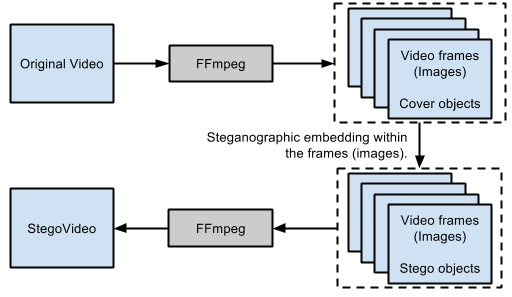
\includegraphics[width=0.9\textwidth]{images/multi.png}}
\caption{Embedding within multiple video formats.}
\label{multi}
\end{figure}

The user specified video is first converted into a sequence of images, one for each frame of the video. Steganographic embedding then occurs within these images before being reassembled back into a video\footnote{The (possible) video audio is extracted separately and then recombined during the assembly process.}. The \texttt{JPEG} file format was chosen for the intermediate frames due to the large number of steganographic algorithms operating on them. \texttt{FFmpeg} facilitates the extraction and assembling of the video frames, allowing this method to work with virtually any video format due to its extensive codec library. Note that the extraction of video frames will be a lossy process, leading to small visible \texttt{JPEG} compression artifacts when comparing the original video and the extracted frames. This is (initially) not a issue for the proposed technique and is not an indication of steganographic embedding. However, the reassembly process cannot be lossy. The data embedded using the identified embedding algorithms operating on \texttt{JPEG} images will not survive recompression. This constraint leads to the following pair of \texttt{FFmpeg} commands shown in listing \ref{extract} and \ref{assembly}.


\begin{lstlisting}[caption={\texttt{FFmpeg} frame extraction command.}, frame=single, label=extract,upquote=true]
ffmpeg -r <video_fps> -i <video_path> -qscale:v 1 -f image2 /tmp/stegasis/image-%d.jpg
ffmpeg -i <video_path> /tmp/stegasis/audio.mp3
\end{lstlisting}

\begin{lstlisting}[caption={\texttt{FFmpeg} video reassembly command.}, frame=single, label=assembly,upquote=true]
ffmpeg -r <video_fps> -i /tmp/stegasis/image-%d.jpg -i /tmp/stegasis/audio.mp3 -codec copy -c:a aac -strict -2 -b:a 192k -shortest output.mkv
\end{lstlisting}

The frame extraction command extracts each frame of the video file using the highest quality setting and writes them as \texttt{JPEGs} to \texttt{/tmp/stegasis/}. The reassembly command \textit{muxes} the modified video frames and audio together into a single \texttt{MKV} file. Note the use of \texttt{-codec copy}, this tells \texttt{FFmpeg} to literally copy the \texttt{JPEGs} into a \textit{Motion JPEG} (\texttt{MJPEG}) stream. This ensures the frames are not recompressed - preserving the embedded data. This process was verified to be correct by noting the \texttt{MD5} hash of the \texttt{JPEG} frames prior to being muxed. These frames were then extracted from the resulting \texttt{MKV} file, their hashes computed and compared.

This method allows \texttt{Stegasis} to operate on an arbitrary video file, but not to remount the produced \texttt{MKV} file. The above paragraph states that the extraction process being lossy is (initially) not a problem. However, if we extract the frames of a produced \texttt{MKV} file using a lossy process, the data embedded within the frames will be damaged. To combat this, a third \texttt{FFmpeg} command is used when remounting an already formatted \texttt{MKV} file, as shown in listing \ref{remount}.

\begin{lstlisting}[caption={\texttt{FFmpeg} \texttt{MKV} \texttt{MJPEG} fram extraction command.}, frame=single, label=remount,upquote=true]
ffmpeg -r <video_fps> -i <video_path> -vcodec copy /tmp/stegasis/image-%d.jpg
\end{lstlisting}

The use of \texttt{-vcodec copy} tells \texttt{FFmpeg} to losslessly extract each \texttt{JPEG} image from the \texttt{MJPEG} stream - preserving the embedded data.

As with the core project, a video decoder performing the above proposed method was implemented satisfying the \texttt{Video Decoder} interface. When \texttt{Stegasis} is run, a check occurs to see whether the provided file is an uncompressed \texttt{AVI}. If it is, the native \texttt{AVI} decoder developed is used. If it is not, the above video decoder is used, allowing \texttt{Stegasis} to operate seamlessly across all video types without the user needing to manually specify which video decoder to use.\\

\noindent
The final step of this method is to implement embedding algorithms operating on \texttt{JPEG} images. Due to the design of \texttt{Stegasis}, by implementing the new algorithms satisfying the \texttt{Steganographic Algorithm} interface, all of the file system logic will continue to work as expected.

The implemented algorithms are all based on the \texttt{JPEG} DCT LSB method (also known as the \textit{JSteg} algorithm) and embed data within the least significant bits of the \texttt{JPEGs} discrete cosine transform coefficients. As with the core project, several versions of the basic algorithm were developed including permuted and encrypted variants, reusing ideas and code from the core implementation. Algorithm \ref{jpegalg} shows pseudocode for the basic embedding algorithm.

\begin{algorithm}
\caption{Basic \texttt{JPEG} embedding algorithm.}
\label{jpegalg}
\begin{algorithmic}[1]
\For{i $\gets$ 0 upto data\_bytes - 1}
	\For{j $\gets$ 7 down to 0}
		\State (row, block, coefficient) $\gets$ getCoefficientForOffset(offset++)
		\State component = 2
		\Comment{Components 2 and 3 are the chroma components.}
		\State row $\gets$ chunk.getRow(row, component)
		\If{ The jth significant bit of data[i] == 1}
			\State Set LSB(row[block][coefficient]) to 1
		\Else
			\State Set LSB(row[block][coefficient]) to 0
		\EndIf
	\EndFor
\EndFor
\end{algorithmic}
\end{algorithm}

Listing \ref{dctp} shows the permuted variant of the implemented \texttt{JPEG} embedding algorithm.\\

\begin{lstlisting}[caption={Permuted \texttt{JPEG} embedding algorithm (\texttt{steg/dctp\_algorithm.cc:48}).}, frame=single, label=dctp,upquote=true,float,floatplacement=!h]
virtual void embed(Chunk *c, char *data, int dataBytes, int offset) {
  int frameByte = lcg.map[offset++];
  int row, block, co, comp;
  JBLOCKARRAY frame; 
  for (int i = 0; i < dataBytes; i ++) {
    for (int j = 7; j >= 0; j --) {
      this->getCoef(frameByte, &row, &block, &co);
      comp = (co % 2) + 1;
      frame = (JBLOCKARRAY)c->getFrameData(row, comp);
      if ((((1 << j) & data[i]) >> j) == 1) {
        frame[0][block][co] |= 1;
      } else {
        frame[0][block][co] &= ~1;
      }
      frameByte = lcg.map[offset++];
    }
  }
};
\end{lstlisting}

The component to embed within is chosen using the calculation \texttt{(co \% 2) + 1}, this will uniformly distribute the embedded data bits between the two chroma components, deliberately not touching the luminance component. 

At higher capacity settings, this embedding algorithm does begin to produce visual artifacts within the video frames. Figure \ref{jpegarti} illustrates this when a capacity setting of 100\% was used.

\begin{figure}[!h]
\centerline{
\includegraphics[width=\textwidth]{images/bb_100cap.png}}
\caption{Embedding artifacts at 100\% capacity.}
\label{jpegarti}
\end{figure}

However, at lower capacity settings it is not possible to visually differentiate between the cover and stego objects\footnote{This claim is verified within the evaluation section \ref{security}.}. Figure \ref{jpegnoart} shows the same frame as above, but using a capacity setting of 20\%. (Left image is the original frame.)

\begin{figure}[!h]
\centerline{
\includegraphics[width=\textwidth]{images/bb_20cap.png}}
\caption{Frame comparison at 20\% capacity.}
\label{jpegnoart}
\end{figure}

\noindent
The \texttt{JEPG} embedding algorithms allow \texttt{Stegasis} to achieve the $>$100\% embedding capacities claimed within the opening paragraph of this document. The reason this is possible is due to the final stage of \texttt{JPEG} compression - ``Encode the resulting coefficients using a Huffman variable word-length algorithm''. This effectively compresses the embedded data before it is written back to disk. To show this in action, listing \ref{200cap} shows a 306 MB file embedded within a 189 MB video.

\begin{lstlisting}[caption={Demonstration of 162\% embedding capacity.}, frame=single, label=200cap]
$ ls -lah
-rw-rw-r-- 1 scott scott 189M Jan 15 22:30 video.mkv
$ stegasis mount -alg=dctl video.mkv /mnt/video
[...]
Mounting...
$ ls -lah /mnt/video
total 4.0K
drwxr-xr-x  2 root root    0 Jan  1  1970 .
drwxrwxrwt 12 root root 4.0K Jan 15 22:26 ..
-rwxr-xr-x  1 root root 306M Jan  1  1970 file1
\end{lstlisting}

The performance of \texttt{Stegasis} using this method is noticeably slower compared to uncompressed \texttt{AVI} files. This is due to the necessary decompressing and recompressing of the \texttt{JPEG} frames. As mentioned in the preparation section, it is not possible to hold all of the decompressed \texttt{JPEG} frames in memory, meaning they will need to remain compressed, only being decompressed when requested. Initially, the \texttt{JPEG} files were left on disk and read into memory and decompressed when requested before being recompressed and written back. This understandably gave terrible performance due to the large amount of disk IO. This was rectified by reading all of the compressed \texttt{JPEG} images into memory upon video mount. The decompression and recompression operates could then operate on this memory - no longer involving any disk IO.\\

\noindent
The above described additions to \texttt{Stegasis} allow it to operate across a large range of video formats, greatly increasing practicality and successfully completing the extension task.

\subsubsection{File system directory structures}

The core implementation of the file system does not allow the creation and manipulation of directories, forcing all files written to the volume to reside in the root. Although \texttt{Stegasis} is still usable with this limitation, it would be nice to allow users to organise their embedded files using directories as you would expect from a normal file system. To achieve this, the \texttt{mkdir} \texttt{FUSE} operation will need to be implemented along with a few changes made to the current file system implementation.

A third data structure, \texttt{dirs} is first added along side \texttt{fileSizes} and \texttt{fileIndex} containing each of the directories within the file system. The \texttt{mkdir} operation is then trivial to implement as shown in listing \ref{dir}.

\begin{lstlisting}[caption={\texttt{FUSE} mkdir implementation (\texttt{fs/stegfs.cc:158}).}, frame=single, label=dir]
int SteganographicFileSystem::mkdir(const char *path, mode_t mode) {
  this->dirs.insert(path);
  return 0;
}
\end{lstlisting}

Changes will have to be made to a few \texttt{FUSE} functions including \texttt{readdir}. It is no longer correct to just iterate over all files in the file system and return their names since you only want to return a file if the function call is requesting the folder that file directly resides within. Consider the following example wherein the file system contains one sub-directory and two files; \texttt{/test.txt}, \texttt{/folder/other.txt}. If \texttt{readdir} requests a path of \texttt{/folder/}, only \texttt{/folder/other.txt} should be returned. This can be accomplished by testing if the requested path is a prefix of the file name. However, this method fails when directories are created within directories - files within sub-directories of the path should not be returned. This is fixed by checking the number of slashes in the file name and comparing this number of slashes in the path. Algorithm \ref{dirs} describes the \texttt{readdir} implementation.

\begin{algorithm}
\caption{Algorithm for the \texttt{readdir} implementation.}
\label{dirs}
\begin{algorithmic}[1]
\State add(`..')
\State add(`.')
\State pathSlashes $\gets$ number of slashes in path
\For{for file in (fileSizes and dirs)}
	\State fileSlashes $\gets$ number of slashes in file
	\If{path == /}
		\If{file contains one slash}
			\State add(file)
		\EndIf
	\ElsIf{path is a prefix of file and pathSlashes == fileSlashes - 1}
		\State add(file)
	\EndIf
\EndFor
\end{algorithmic}
\end{algorithm}

Changes will now need to be made to write the directories to the video file and to read them back, preserving the directory structure between unmounts and remounts. It was chosen to represent a directory as a file in the header of the video which has a value of $-1$ in the \texttt{number of triples} field. The \texttt{readHeader} and \texttt{writeHeader} functions were modified appropriately.

These changes successfully implement the extension task and greatly improve the usability of the file system. With the exception of permissions and access and modification times, \texttt{Stegasis} now provides all the functionality one would expect from a typical file system.

%unlink doesnt work check for dirs...
%also have i implemented mv??

\subsubsection{Plausible deniability}

Similar to \texttt{TrueCrypts} hidden volume feature, I planned to implement plausible deniability by embedding two separate file systems within one video, each using different user provided passphrases. The \textit{outer} volume will reside at the beginning of the video (where it usually would) and the user should populate this volume with files they are willing to have seen. The \textit{inner} volume will reside half way through the video file and the user should place sensitive files within here. When forced to give up the encryption keys, the user can reveal the passphrase for the outer volume in confidence the inner volume will not be compromised.

This method is vulnerable to steganalysis attacks that would be able to detect the presence of the hidden volume half way through the video. To combat this, random data is embedded throughout the entire video during the format process. Since the volumes are encrypted, it will not be possible to tell if the identified embedded data is a hidden volume or just the random data written during the formatting process.

The modifications to \texttt{Stegasis} required to implement this feature were surprisingly simple. A second passphrase command line flag \texttt{pass2} was added, if this is specified during the format process random data is written to each frame of the video and two headers written at the start and in the middle of the video. The mount process will now attempt to extract and decrypt the first header using the provided passphrase. If this fails, it then attempts to decode the second header (embedded within the middle frame). Depending on which header extracts successfully, the outer or hidden file system is presented to the user.

Listing \ref{deny} shows an example use case of the plausible deniability functionality.

\begin{lstlisting}[caption={\texttt{Stegasis} plausible deniability functionality.}, frame=single, label=deny]
$ stegasis format -alg=lsba -pass=outer -pass2=hidden /media/Backup/video.avi
[...]
Format successful!
$ stegasis mount -alg=lsba -pass=outer /media/Backup/video.avi /tmp/steg
[...]
Mounting...

[Second Terminal]
$ echo 'outer' > /tmp/steg/outer.txt

[First Terminal]
<Control-C>
[...]
$ stegasis mount -alg=lsba -pass=hidden /media/Backup/video.avi /tmp/steg
[...]
Mounting...

[Second Terminal]
$ echo 'inner' > /tmp/steg/sensitivefile.txt
\end{lstlisting}

Since the header and data for the hidden file system is stored within the middle video frame onwards, it is possible to damage it by writing too much data to the outer volume, thus overwriting the hidden volume header. The user has sacrificed half of the total embedding capacity in return for plausible deniability.

\subsubsection{Hiding data within audio}

It is stated within the project proposal that ``a substantial part of an \texttt{AVI} file may be the audio data''. I was correct to use the word ``may'' within this statement since it turns out that a very small percentage of an uncompressed \texttt{AVI} file is the audio data. Similarly low percentages apply to other video formats due to modern audio compression algorithms such as \texttt{MP3}. The question of how this extra embedding capacity could actually be utilised is also quite prevalent since \texttt{Stegasis} and the file system logic all rely on the idea of the video being broken up into frames. This concept does not translate easily over to audio. It was therefore deemed not worth perusing this extension task. 

\subsubsection{Evaluation of embedding impact on video quality}

To evaluate the requirement ``Embedding should occur with no perceivable impact on video quality.'', a web application was required to be developed and hosted. Figure \ref{site} shows a screenshot of the finished website hosted at \texttt{www.stegasis.co.uk} for the majority of the duration of the project.

\begin{figure}[!h]
\centerline{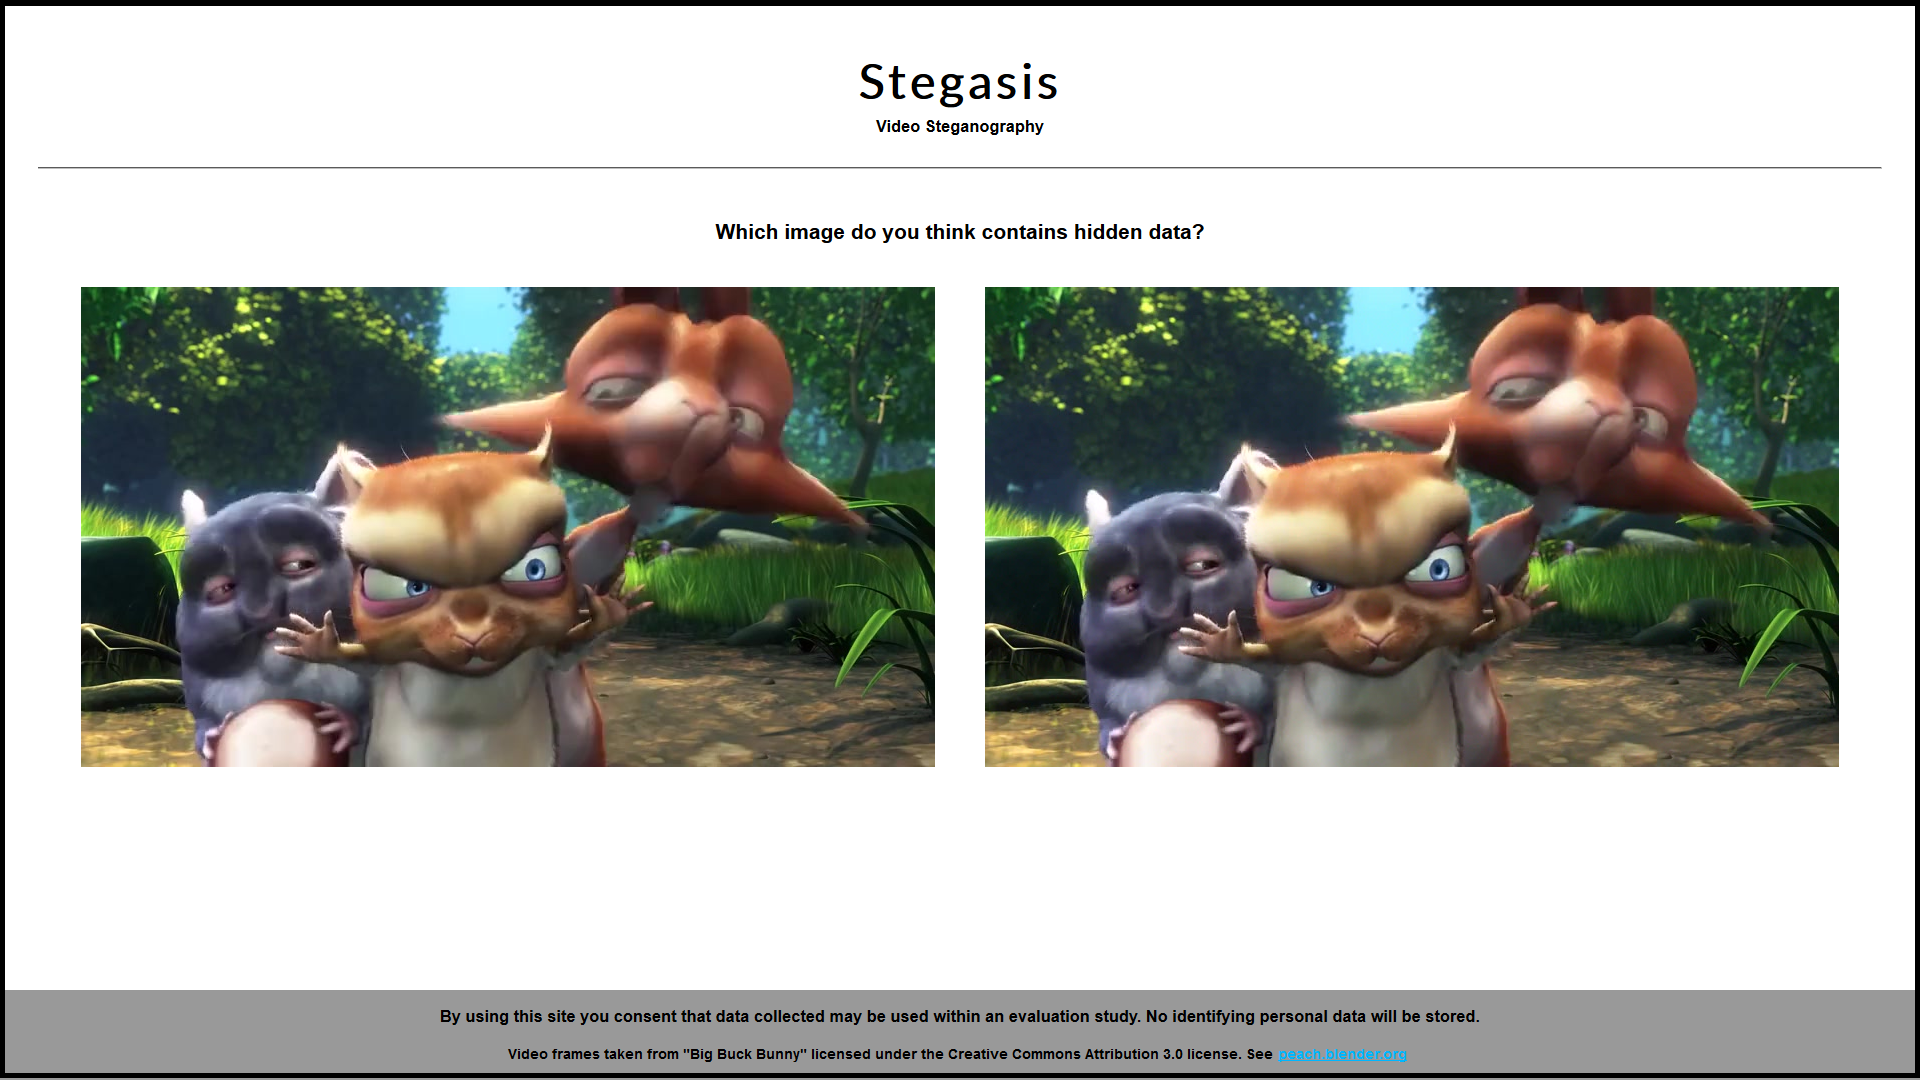
\includegraphics[width=\textwidth]{images/site.png}}
\caption{Screen shot of the evaluation study site.}
\label{site}
\end{figure}

The user is presented with two images and asked the question ``Which image do you think contains hidden data?''. The user may inspect the image for as long as they wish, and by clicking on an image, they then select their choice.

In total there are 14,912 pairs of images, one of which is randomly selected for each page load. One of the images is the original video frame while the other has 2.5 kB of data embedded within it using the permuted \texttt{JPEG} embedding algorithm and a capacity setting of 20\% (the default value). The position of the ``correct'' image is randomly chosen and the file names of the images are also random strings. This tries to thwart any attempts at foul play, possibly damaging the collected results. When a user first visits the site, a cookie containing a unique ID is issued allowing data points from the same user to be aggregated together.\\

\noindent
The results of this evaluation study obtained by the implemented web application are discussed in section \ref{security} and give a definitive answer to the question of perceivable embedding impact.

\subsection{Testing}
\label{testing}

\texttt{Stegasis} was tested using a combination of unit, integration and visual testing. Due to the decoupled nature of the steganogrphic embedding algorithms, it was easy to produce unit tests for the embedding and extraction functionality. A total of *largenumber* test cases were written testing all 11 embedding algorithms and associated code. Listing \ref{unittest} gives an example unit test.

\begin{lstlisting}[caption={Embedding algorithm unit test (\texttt{steg/steg\_algorithm\_test.cc:100}).}, frame=single, label=unittest]
int SteganographicFileSystem::mkdir(const char *path, mode_t mode) {
  this->dirs.insert(path);
  return 0;
}
\end{lstlisting}

The above unit test verifies the steganogrphic correctness of the stego systems, checking that data embedded using a key \textbf{k} is correctly extracted when using the same key.

It was deemed more appropriate to test the file system functionality via an integration test suite due to its highly coupled nature. The test suite revolved around a number of compressed archives containing test files and directory structures. \texttt{Stegasis} is first instructed to mount a test video into \texttt{/tmp/test}. These archives are then copied into the file system and uncompressed. Once the extraction process has completed, the resulting file system is traversed to check the contents is as expected. Visual testing was also employed. For example, large media content such as high definition video was copied into the mounted volume and checked to see if it played back correctly. This is a good test case since the file (due to its size) will be spread across a large proportion of the video. Indeed, several bugs were identified using this testing approach.

The \texttt{AVI} parser was tested using a black box testing approach on a number of different uncompressed \texttt{AVI} videos. The parser prints out debug information about the video file which can be visually inspected. For example, the resolution of the video contained within the \texttt{BITMAPINFOHEADER} can be compared against the known value. Checking that the \texttt{AVI} still plays back after steganographic modification is also a good indication that the parser is operating successfully.

See the appendix section \ref{app:codetest} for some more testing code samples. 

\section{Evaluation}
\subsection{Satisfaction of Requirements}

As stated in the preparation section, the project will be considered a success if all of the core requirements have been satisfied. Each requirement will now be addressed in turn.

\subsubsection{Embedding data within video files}

\texttt{Stegasis} does indeed allow data to be embedded within video files. Furthermore, it provides a total of 10 steganogrphic embedding algorithms all of which satisfy correctness\footnote{Verified by one of the unit test cases as explained in section \ref{testing}.} and, after an evaluation study discussed in section \ref{security} below, it was concluded that \texttt{Stegasis} operates with no perceivable impact on video quality. A number of steganalysis tools were indeed developed and tested the security of the proposed stego systems, prompting the design of more secure embedding algorithms. Encryption functionality is also provided making use of a user provided passphrase. Finally, a capacity setting was also implemented allowing users to choose a trade off between steganographic security and embedding capacity. This satisfies all points of the first requirement.

\subsubsection{Providing a file system interface}

\texttt{Stegasis} also successfully satisfies the second requirement. Users can specify a mount point at which the volume will be mounted and data written to and read from this volume will embedded and extracted from the video on the fly. Standard Unix tools including \texttt{cp}, \texttt{mv} and \texttt{rm} work as expected and the file system is correctly persevered between unmounts and remounts of the same video.

\subsubsection{Supporting uncompressed AVI}

Raw uncompressed \texttt{AVI} files are supported via a developed native parser which allows access to and modification of individual pixel data, therefore fulfilling the third requirement.

\subsubsection{File system performance}

The performance of the file system allows full HD video content to be played back from directly within the volume, meeting the first point of this requirement. The second point was harder to satisfy; achieving read and write speeds in excess of 20 MB/s was not a trivial task. The file system does manage to provide read and write speeds in excess of 30 MB/s (and under ideal conditions\footnote{These conditions are discussed below in section \ref{perf}.}, these speeds can reach 160MB/s.), but only for the algorithms which do not encrypt the embedded data and only if the performance flag (\texttt{-p}) has been specified. Since read and write speeds in excess of 20 MB/s can be provided by the file system, I consider this requirement satisfied. Performance is discussed in more detail below in section \ref{perf}.\\

\noindent
\texttt{Stegasis}, having satisfied all of the core requirements can therefore be considered a success. The extension task requirements are now discussed individually. 

\subsubsection{Supporting multiple video formats}

The novel method described in section \ref{extffmpeg} allows \texttt{Stegasis} to seamlessly operate across virtually every video format available today, including the explicitly mentioned \texttt{MP4} format. The implemented embedding algorithms operating on \texttt{JPEG} images enable very large embedding capacities allowing multiple large files to hidden inside of a single video file.

\subsubsection{File system directory operations}

Directory functionality was successfully implemented allowing the creation and manipulation of directory structures, enabling users to organise their files within folders. The \texttt{mv} and \texttt{rm} commands work as expected when operating on directories as well as normal files. 

\subsubsection{Embedding within audio}

This extension task was investigated but was decided not to be implemented due to the relativity little embedding capacity gain compared to the work required to implement it.

\subsubsection{Plausible deniability}


Haven't done this yet.

\subsubsection{Evaluation of the visual impact of embedding}

A website was implemented and hosted for the majority of the duration of the project. A total of 2057 data points were collected from 21 unique users. The results are discussed below in section \ref{security}, and the outcome of the study confirms that it is not possible to visually differentiate videos produced by \texttt{Stegasis} when using the default capacity setting (20\%). This satisfies the final extension task.\\

\noindent
\texttt{Stegasis} therefore has also satisfied all\footnote{I am considering the audio extension task satisfied since it was investigated and chosen not to be implemented.} of the proposed extension tasks, further cementing the success of the project.

\subsection{Security}
\label{security}

Although security of the embedding algorithms was not a major focus of this project, steganalysis techniques were implemented and these led to more secure algorithms being developed. The evaluation user study was also focused on security - attempting to decide if it is possible to visually differentiate between cover and stego objects produced by \texttt{Stegasis} when using its default capacity setting of 20\%. The results of this study are now statistically analysed to give an answer to this question.

It is first noted that if a user cannot tell the difference between the two presented images, they will select one at random. From the phrasing of the question posed to the user, a response is considered correct if the image selected did contain hidden data and incorrect if it did not. If a user were to randomly guess each time, the resulting data stream would be a random stream of corrects and incorrects. Letting correct be represented as 1 and incorrect as 0, this stream of random corrects and incorrects becomes a random bit string. Therefore, if it can be shown that the collected data is a random bit string, it can then be concluded that the users must have been randomly guessing and therefore could not differentiate between the two presented images.

To determine if the obtained bit string is in fact random, a number of statistical randomness tests are used, provided by \texttt{ent}\textsuperscript{\cite{ent}}, a pseudorandom number sequence test program. Listing \ref{entout} shows the output of \texttt{ent} when applied to the bit string.

\begin{lstlisting}[caption={Output of \texttt{ent}.},frame=single, upquote=true,label=entout,showstringspaces=false]
Entropy = 0.999664 bits per bit.

Optimum compression would reduce the size
of this 2040 bit file by 0 percent.

Chi square distribution for 2040 samples is 0.95, and randomly
would exceed this value 33.00 percent of the times.

Arithmetic mean value of data bits is 0.5108 (0.5 = random).
Monte Carlo value for Pi is 3.523809524 (error 12.17 percent).
Serial correlation coefficient is -0.035776 (totally uncorrelated = 0.0).
\end{lstlisting}

These results strongly indicate that the bit string is random. Quoting the \texttt{ent} web page ``The chi-square test is the most commonly used test for the randomness of data [...] If the percentage is greater than 99\% or less than 1\%, the sequence is almost certainly not random. If the percentage is between 99\% and 95\% or between 1\% and 5\%, the sequence is suspect. Percentages between 90\% and 95\% and 5\% and 10\% indicate the sequence is ``almost suspect''. [...] A chi-square result of a genuine random sequence created by timing radioactive decay events: Chi square distribution for 500000 samples is 249.51, and randomly would exceed this value 40.98 percent of the times.''

I feel this is enough evidence to conclude the bit string is random enough and therefore that the users within the evaluation study could not differentiate between the stego and cover images.

Although we have concluded that \texttt{Stegasis} can operate with no perceivable visual impact on video quality, this does not imply that it will resist further steganalysis techniques. Indeed, the \textit{Histogram attack} which operates on \texttt{JPEG} images breaks the stego systems implemented in the multiple video formats extension task (even using low capacity settings). The histogram attack enumerates the frequencies of the DCT coefficients of a given image. A characteristic of unmodified \texttt{JPEG} images is that its histogram is symmetrical about 0, that is, coefficients $n$ and $-n$ have roughly equal frequencies. This characteristic is lost when embedding occurs. Figure \ref{hist} shows the effectiveness of the attack, comparing the histogram of an original video frame to one with embedded data. It clearly manages to differentiate between the cover and stego objects.

\begin{figure}[!tbh]
\centerline{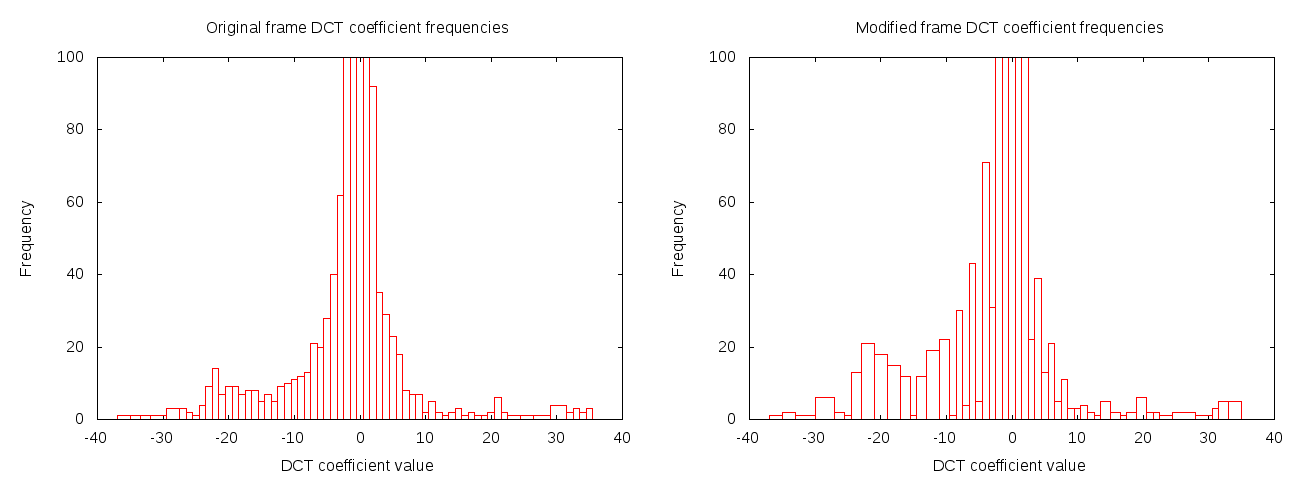
\includegraphics[width=\textwidth]{images/hist.png}}
\caption{The histogram attack.}
\label{hist}
\end{figure}

This does lead to the unfortunate conclusion that the steganography provided by \texttt{Stegasis}, as it stands, is broken - a steganalyst would be able to conclude with relative ease that videos produced by \texttt{Stegasis} contained hidden data. I do not believe however that this renders \texttt{Stegasis} useless. The embedding algorithms employing cryptography ensure that even if the embedded data is identified, it cannot be extracted nor decrypted. Furthermore, the plausible deniability functionality provided by \texttt{Stegasis} keeps sensitive information safe even if users are forced to give up encryption keys. Also note that the video file in question would have had to have been specifically targeted for these attacks to occur\footnote{For example, I do not believe automated steganalysis occurs for all video files emailed or uploaded to file sharing websites.}.

With the above said, it would be a straight forward process to incorporate more secure embedding algorithms which do resist the histogram attack (such as F5 and OutGuess) due to the framework \texttt{Stegasis} already provides.

\subsection{Performance}
\label{perf}

The performance of \texttt{Stegasis}, and in particular the file system, is very important to consider. As with \texttt{TrueCrypt}, using \texttt{Stegasis} should constitute? a similar experience to copying files onto removable storage. 

\subsubsection{Performance of the file system}

Due to the large embedding capacities offered, large files are expected to be copied into the file system and therefore embedded into the video. The write performance of the file system was therefore given a lot of attention during the implementation. The biggest improvement in file system performance was obtained by enabling the \texttt{FUSE} \texttt{big\_writes} mount option. By default, \texttt{FUSE} limits write calls to blocks of 4096 bytes. \texttt{big\_writes} allows this limit to be increased to a maximum of 128 kB. Figure \ref{writeper} shows the effect of varying the block size on write performance for the LSB embedding algorithm (with the \texttt{-p} flag).

\begin{figure}[!tbh]
\centerline{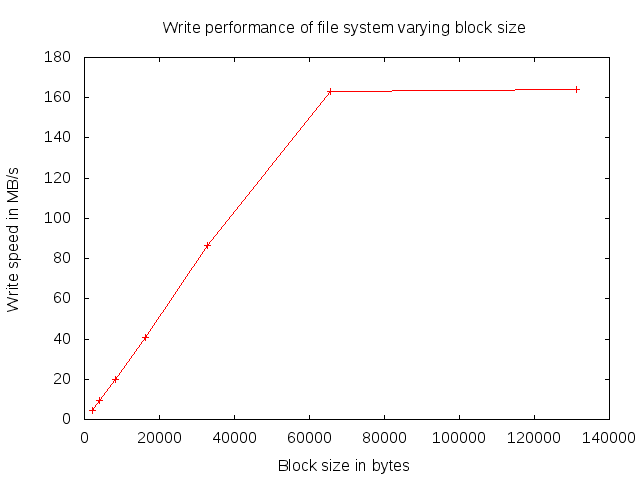
\includegraphics[width=\textwidth]{images/writeper.png}}
\caption{Write performance whilst varying block size.}
\label{writeper}
\end{figure}

The data points for the graph were obtained using the command line tool \texttt{dd} as shown in the listing below. Note that this test provides ideal conditions, having a large block size and writing all zeros - most use cases will not be like this.

\begin{lstlisting}[caption={Testing the file system performance using \texttt{dd}.}, frame=single, label=dd,float,floatplacement=!htH]
$ dd if=/dev/zero of=test bs=128k count=610
610+0 records in
610+0 records out
79953920 bytes (80 MB) copied, 0.456444 s, 175 MB/s
\end{lstlisting}

To evaluate the file system performance under more standard conditions, I timed the copying of an 80 MB video file into and out of the file system using the \texttt{time} tool. This process was repeated multiple time and an average taken giving an average write speed of 33.6 MB/s and read speed of 46.3 MB/s. This is significantly slower than above, but is still on par with USB 3.0 device speeds\textsuperscript{\cite{usb3}}, surpassing the performance requirement. As expected, the embedding algorithms which permute and encrypt data give worse file system performance, but I think this is a fair trade off.

\subsubsection{Performance of video formatting}

Another area worth considering is the time \texttt{Stegasis} takes to format video files. Although it is hard to quantify a ``good'' format time, I would expect a time of under 1 minute to be reasonable for an average 5 minute video. The format time of \texttt{AVI} files is more dependent on disk read performance, whereas for other video formats, processor performance will be more important (due to the video transcoding involved). I measured the time taken to format a variety of video files on my desktop computer. The results are summarised in table \ref{formatres} below.

\begin{table}[h]
\centering
\begin{tabular}{|c|c|c|lll}
\cline{1-3}
\textbf{Video file} & \textbf{Volume capacity (MB)} & \textbf{Format Time (seconds)}      \\ \cline{1-3}
700 MB 10 second \texttt{AVI} & 96.60 & 6.146   \\ \cline{1-3}
14 MB 3 minute \texttt{MP4} & 28.98 & 13.143   \\ \cline{1-3}
34 MB 4 minute \texttt{MP4} & 159.07 & 29.270   \\ \cline{1-3}
80 MB 18 minute \texttt{FLV} & 55.63 & 45.810  \\ \cline{1-3}
\end{tabular}
\caption{Video format times}
\label{formatres}
\end{table}

\section{Conclusions}

Informally, I wanted this project to result in the ``\texttt{TrueCrypt} of video steganography'' focusing on a practical application allowing multiple files to be easily steganographically embedded within video files utilising a file system interface. This involved researching multiple technical fields (mainly Steganography, file systems and video formats) and developing an application to combine them all into a polished tool.

A number of steganographic embedding algorithms were researched and implemented borrowing ideas and algorithms from cryptography to further increase security. A file system in user space residing within a video file was designed and implemented offering the majority of the functionality one would expect from a standard file system. A native \texttt{AVI} parser was developed along with a novel method of supporting other video formats utilising \texttt{FFmpeg}. Finally a Linux command-line application, \texttt{Stegasis}, was produced combining the above into a single application.

\texttt{Stegasis} satisfies all of the core project requirements and implements all of the proposed extension tasks. In reference to the evaluation section of this document, I very much consider this project a success and hope to release \texttt{Stegasis} in the near future.

\subsection{Lessons Learnt}

The ``Launch early, iterate often'' approach taken to development did come with some drawbacks. Most notably, design decisions made early on during development were sometimes not given as much thought as they possibly should have. This resulted in some issues arising much later during development which required a lot of work to correct. Had due thought been given to these decision at the start of the development process, a large amount of time spent refactoring code could have been saved. 

\subsection{Future Project Directions}

As discussed in the evaluation section, \texttt{Stegasis} currently lacks secure steganographic embedding algorithms. Further work would therefore likely involve implementing more secure embedding algorithms. Another avenue to explore would be implementing more native video decoders. For example, a native \texttt{MP4} decoder could be produced which embedded data within motion vectors. This has an advantage over the \texttt{FFmpeg} method since a new, \texttt{MKV} video is not produced - the \texttt{MP4} would be modified in place as occurs with \texttt{AVI} files.
Finally, it would be great for \texttt{Stegasis} to be cross platform. Developing a Linux only application severely limits the target audience. However, since the file system was implemented using \texttt{FUSE} (which is not compatible with Windows) this may prove tricky.

\vfill

\pagebreak

\begin{thebibliography}{1}

\bibitem{digmedia} \emph{Steganography in Digital Media}, Jessica Fridrich 2010, pp. xv - xvi

\bibitem{uklaw} \emph{Contested UK encryption disclosure law takes effect}, Jeremy Kirk 2007, Washington Post\\ 
\path{www.washingtonpost.com/wp-dyn/content/article/2007/10/01/AR2007100100511.html}

\bibitem{digmedia2} \emph{Steganography in Digital Media}, Jessica Fridrich 2010, p. xvii

\bibitem{survey} \emph{A Survey of Steganographic and Steganalytic Tools for the Digital Forensic Investigator}, Pedram Hayati et al.\\
\path{www.pedramhayati.com/images/docs/survey_of_steganography_and_steganalytic_tools.pdf}

\bibitem{truecrypt} \emph{TrueCrypt is a source-available freeware utility used for on-the-fly encryption.}\\
\path{www.truecrypt.org}

\bibitem{nsa} \emph{The NSA Thinks You Are an Extremist If You Care About Privacy}, Fahmida Rashid 2014, PCMag\\
\path{securitywatch.pcmag.com/privacy/325273-the-nsa}

\bibitem{prisoner} \emph{The prisoners' problem and the subliminal channel}, Gustavus Simmons 1984, Advances in Cryptology, pp. 51 - 67

\bibitem{kirc} \emph{La Cryptographie Militaire}, Auguste Kerckhoffs 1883

\bibitem{steganalysis} \emph{Steganalysis: The Investigation of Hidden Information}, Neil Johnson and Sushil Jajodia 1998 

\bibitem{avicommon} \emph{Using Video Data}, ATLAS.ti 6 2011\\
\path{atlasti.com/wp-content/uploads/2014/05/video_formats.pdf}

\bibitem{aviformat} \emph{AVI RIFF File Reference}, Microsoft\\
\path{msdn.microsoft.com/en-us/library/windows/desktop/dd318189\%28v=vs.85\%29.aspx}

\bibitem{jpegsteg} \emph{Steganography and Steganalysis of JPEG Images}, Mahendra Kumar\\
\path{www.cise.ufl.edu/~makumar/proposalppt.pdf}

\bibitem{jsteg} \emph{JSteg: Steganography and Steganalysis}, Murali P 2009\\
\path{csis.bits-pilani.ac.in/faculty/murali/netsec-09/seminar/refs/anuroopsrep.pdf}

\bibitem{outguess} \emph{Hide and Seek: An Introduction to Steganography}, Niels Provos and Peter Honeyman 2003, p. 36\\
\path{niels.xtdnet.nl/papers/practical.pdf}

\bibitem{f5} \emph{F5 — A Steganographic Algorithm}, Andreas Westfeld\\
\path{www2.htw-dresden.de/~westfeld/publikationen/f5.pdf}

\bibitem{libjpeg} \emph{Libjpeg, a widely used C library for reading and writing JPEG image files}\\
\path{libjpeg.sourceforge.net}

\bibitem{sensitive} \emph{Human eye sensitivity and photometric quantities}\\
\path{www.ecse.rpi.edu/~schubert/Light-Emitting-Diodes-dot-org/Sample-Chapter.pdf}

\bibitem{ffmpeg} \emph{FFmpeg: A complete, cross-platform solution to record, convert and stream audio and video}\\
\path{www.ffmpeg.org}

\bibitem{ffmpegcodec} \emph{FFmpeg Codecs Documentation}\\
\path{www.ffmpeg.org/ffmpeg-codecs.html}

\bibitem{fuse} \emph{FUSE: File system in userspace}\\
\path{fuse.sourceforge.net}

\bibitem{fuseper} \emph{Linus vs FUSE: Kernel file system vs FUSE}, Sage 2011\\
\path{ceph.com/dev-notes/linus-vs-fuse}

\bibitem{stegostick} \emph{Stegostick: A steganographic Tool that lets you hide any file into any file}, 2008\\
\path{sourceforge.net/projects/stegostick}

\bibitem{stegomagic} \emph{Stegomagic: An encrypting software application designed specifically for helping you hide files or messages in media items}, 2014\\
\path{www.softpedia.com/get/Security/Encrypting/StegoMagic.shtml}

\bibitem{tcsteg} \emph{Real steganography with TrueCrypt}, Martin Fiedler 2011\\
\path{keyj.emphy.de/real-steganography-with-truecrypt}

\bibitem{stegovideo} \emph{Stegovideo: A unique tool for hiding information in video}, Oleg Petrov 2011\\
\path{www.compression.ru/video/stego_video/index_en.html}

\bibitem{openpuff} \emph{OpenPuff: A steganography tool supporting many carrier formats}, EmbeddedSW\\
\path{embeddedsw.net/OpenPuff_Steganography_Home.html}

\bibitem{steganosaurus} \emph{Steganosaurus is a dissertation project exploring the application of video steganographic and video steganalysis techniques.}, James Ridgway 2014\\
\path{www.steganosaur.us}

\bibitem{bitrate} \emph{YouTube Advanced encoding settings.}, Google 2014\\
\path{support.google.com/youtube/answer/1722171?hl=en-GB}

\bibitem{usb2} \emph{Example USB 2.0 flash drive}, Ebuyer 2015\\
\path{www.ebuyer.com/543103-toshiba-transmemory-8gb}

\bibitem{javafuse} \emph{JavaFUSE provides Java bindings for FUSE}, Aditya Rajgarhia 2010\\
\path{code.google.com/p/javafuse/}

\bibitem{turbojpeg} \emph{TurboJPEG: A Java interface for libjpeg-turbo}\\
\path{www.libjpeg-turbo.org}

\bibitem{javaper1} \emph{Numeric performance in C, C\# and Java}, Peter Sestoft 2010\\
\path{www.itu.dk/people/sestoft/papers/numericperformance.pdf}
 
\bibitem{javaper2} \emph{Time Comparing between Java and C++ Software}, As’ad Mahmoud Alnaser et al. 2012\\
\path{www.scirp.org/journal/PaperDownload.aspx?paperID=21960}
 
\bibitem{javaper3} \emph{A Java vs. C++ performance evaluation: a 3D modeling benchmark}, L. Gherardi et al.\\
\path{www.best-of-robotics.org/pages/publications/gherardi12java.pdf}

\bibitem{iterate} \emph{Release Early, Release Often}, Eric S. Raymond \\
\path{www.catb.org/~esr/writings/cathedral-bazaar/cathedral-bazaar/ar01s04.html}

\bibitem{inver} \emph{The Dependency Inversion Principle}\\
\path{www.objectmentor.com/resources/articles/dip.pdf}

\bibitem{chi} \emph{Attacks on Steganographic Systems: Breaking the Steganographic Utilities EzStego, Jsteg, Steganos, and S-Tools and Some Lessons Learned}, Andreas Westfeld and Andreas Pfitzmann 2000

\bibitem{lcg} \emph{The Linear Congruential Method}, Donald Knuth, The Art of Computer Programming, Volume 2

\bibitem{hull} \emph{Random number generators}, T E. Hull A. R. Dobell 1962

\bibitem{keyd} \emph{PKCS \#5: Password-Based Cryptography Standard}, RSA Laboratories.

\bibitem{pool} \emph{The Whirlpool Secure Hash Function}, Williams Stallings 2006\\
\path{www.seas.gwu.edu/~poorvi/Classes/CS381_2007/Whirlpool.pdf}

\bibitem{ent} \emph{Ent: A Pseudorandom Number Sequence Test Program}, John Walker 2008\\
\path{www.fourmilab.ch/random}

\bibitem{usb3} \emph{Lexar 8GB USB 3.0 JumpDrive}, Ebuyer 2015\\
\path{www.ebuyer.com/399229-lexar-8gb-jumpdrive}

\vfill

\end{thebibliography}

\pagebreak

\appendix
\section{Details of the AVI file format}
\label{app:avi}

\subsection{Detailed AVI form}

Listing \ref{aviform} shows an expanded form of the \texttt{AVI} structure.

\begin{lstlisting}[language=C, caption={Detailed \texttt{AVI RIFF} form}, frame=single, upquote=true,label=aviform,showstringspaces=false]
RIFF (
  'AVI '
  LIST (
    'hdrl'
    'avih'(<Main AVI Header>)
    LIST (
      'strl'
      'strh'(<Stream header>)
      'strf'(<Stream format>)
      [ 'strd'(<Additional header data>) ]
      [ 'strn'(<Stream name>) ]
      ...
    )
    ...
  )
  LIST (
    'movi'
    {SubChunk | 
      LIST (
        'rec '
        SubChunk1
        SubChunk2
        ...
        )
      ...
    }
    ...
  )
  ['idx1' (<AVI Index>) ]
)
\end{lstlisting}

\subsection{The AVI header}

Listing \ref{aviheader} shows the definition of the main \texttt{AVI} header.

\begin{lstlisting}[caption={The \texttt{AVIMAINHEADER} structure.},frame=single, upquote=true,label=aviheader,showstringspaces=false]
typedef struct _avimainheader {
  char     fcc[4];
  int32_t  cb;
  int32_t  dwMicroSecPerFrame;
  int32_t  dwMaxBytesPerSec;
  int32_t  dwPaddingGranularity;
  int32_t  dwFlags;
  int32_t  dwTotalFrames;
  int32_t  dwInitialFrames;
  int32_t  dwStreams;
  int32_t  dwSuggestedBufferSize;
  int32_t  dwWidth;
  int32_t  dwHeight;
  int32_t  dwReserved[4];
} AVIMAINHEADER;
\end{lstlisting}


\section{Stegasis example use} 
\label{app:steg}

\subsection{Stegasis usage information}

Listing \ref{usage} shows the information displayed to the user when the program is run with no (or incorrect) arguments supplied.

\begin{lstlisting}[caption={\texttt{Stegasis} usage information.},frame=single, upquote=true,label=usage,showstringspaces=false]
   _____ _                                  
  / ____| |                     (_)         
 | (___ | |_ ___  __ _  __ _ ___ _ ___      
  \___ \| __/ _ \/ _` |/ _` / __| / __|  
  ____) | ||  __/ (_| | (_| \__ \ \__ \ 
 |_____/ \__\___|\__, |\__,_|___/_|___/ 
                  __/ | v2.1a               
                 |___/                      

Stegasis usage:
  stegasis <command> [-p,-f] -alg=<alg> -pass=<pass> -cap=<capacity> <video_path> <mount_point>
-----------------------------------------------------------------
Example useage:
  stegasis format --alg=lsbk --pass=password123 --cap=50 /media/video.avi
  stegasis mount --alg=lsbk --pass=password123 /media/video.avi /tmp/test
Commands:
  format  Formats a video for use with stegasis
  mount  Mounts a formatted video to a given mount point
Required Flags:
  -alg  Embedding algorithm to use, see below
  -cap  Percentage of frame to embed within in percent
Optional flags:
  -pass  Passphrase used for encrypting and permuting data
  -pass2 Passphrase used for encrypting and permuting the hidden volume
  -p  Do not flush writes to disk until unmount
  -f  Force the FFmpeg decoder to be used
Embedding Algorithms:
  Uncompressed AVI only:
    lsb:  Least Significant Bit Sequential Embedding
    lsbk:  LSB Sequential Embedding XORd with a psudo random stream
    lsbp:  LSB Permuted Embedding using a seeded LCG
    lsb2:  Combination of lsbk and lsbp
    lsba:  LSB Permuted Embedding encrypted using AES
    
  Other video formats:
    dctl:  LSB Sequential Embedding within DCT coefficients
    dctp:  LSB Permuted Embedding within DCT coefficients
    dct2:  Combination of dctp and lsbk
    dcta:  LSB Permuted Embedding encrypted with AES
    dct3:  LSB Permuted Embedding encrypted with AES->Twofish->Serpent
\end{lstlisting}

\subsection{Example use case}

Listing \ref{usecase} shows an example use of \texttt{Stegasis}, formatting and mounting a video with complete command line output.

\begin{lstlisting}[caption={\texttt{Stegasis} example use.},frame=single, upquote=true,label=usecase,showstringspaces=false]
$ stegasis format -alg=lsbp -pass=hunter2 -cap=20 /media/Backup/video.avi 
   _____ _                                  
  / ____| |                     (_)         
 | (___ | |_ ___  __ _  __ _ ___ _ ___      
  \___ \| __/ _ \/ _` |/ _` / __| / __|  
  ____) | ||  __/ (_| | (_| \__ \ \__ \ 
 |_____/ \__\___|\__, |\__,_|___/_|___/ 
                  __/ | v2.1a               
                 |___/                      
Filesize: 776143108
Totalframes: 280
Width: 1280
Height: 720

Reading AVI chunks...
100% [==================================================]
Finished parsing AVI file

Volume capacity: 19.32MB

Writing back to disc...
100% [==================================================]
Format successful!

$ stegasis mount -alg=lsbp -pass=hunter2 /media/Backup/video.avi /tmp/steg
   _____ _                                  
  / ____| |                     (_)         
 | (___ | |_ ___  __ _  __ _ ___ _ ___      
  \___ \| __/ _ \/ _` |/ _` / __| / __|  
  ____) | ||  __/ (_| | (_| \__ \ \__ \ 
 |_____/ \__\___|\__, |\__,_|___/_|___/ 
                  __/ | v2.1a               
                 |___/                      
Filesize: 776143108
Totalframes: 280
Width: 1280
Height: 720

Reading AVI chunks...
100% [==================================================]
Finished parsing AVI file

Header: STEG
Mounting...

[Second Terminal]
$ cd /tmp/steg
/tmp/steg$ cp ~/vid.mp4 .

[Stegasis Terminal]
Embeding, Frame: 203, Size: 36158, Offset: 0
Compacting header...
100% [==================================================]
Writing back to disc...
100% [==================================================]

[Second Terminal]
/tmp/steg$ ls -lah
total 4.0K
drwxr-xr-x  2 root root    0 Jan  1  1970 .
drwxrwxrwt 10 root root 4.0K Jan 15 21:59 ..
-rwxr-xr-x  1 root root  14M Jan  1  1970 lba2.mp4

[Stegasis Terminal]
<Control-C>
Unmounting...
Compacting header...
100% [==================================================]
Writing back to disc...
100% [==================================================]
Successfully unmounted
\end{lstlisting}

\section{Detailed Code samples} 
\label{app:code}

This section contains select detailed code samples.

\subsection{Chi-Squared attack}
\label{app:chi}

Listing \ref{chipy} shows an implementation of the Chi-Squared attack in Python which operates on the \texttt{PPM} image format.

\begin{lstlisting}[language=Python,caption={Chi-Squared attack Python implementation.}, frame=single,label=chipy,showstringspaces=false,upquote=true]
from scipy import integrate, special

file_bytes = open(sys.argv[1], 'rb').read()

header = file_bytes[:2]
if header != 'P6':
  print 'File is not a P6 ppm.'
  sys.exit(0)

fp = 3
width = ''
while True:
  b = file_bytes[fp]
  fp += 1
  if b == ' ':
      break
  width += b

height = ''
while True:
  b = file_bytes[fp]
  fp += 1
  if b == ' ':
      break
  height += b

max_pixel_val = ''
while True:
  b = file_bytes[fp]
  fp += 1
  if b == ' ':
      break
  max_pixel_val += b

output = [0]*100

# fp is now on the first pixel red byte
frameStart = fp
for h in range(1, 100):
  fp = frameStart
  totalPixels = math.floor((h/100.0)*int(width)*int(height))
  X = [0]*(128*3) # X[k] = frequency(2k)
  Y = [0]*(128*3) # Y[k] = frequeincy(2k+1)
  Z = [0.0]*(128*3)

  # Populate the frequency arrays
  end = fp + totalPixels*3
  while fp < end:
      b = ord(file_bytes[fp])
      if b % 2 == 0:
          X[b/2] += 1
      else:
          Y[(b-1)/2] += 1
      fp += 1

   # Calculate theoretically expected frequency
  for i in range(len(Z)):
      Z[i] = (X[i] + Y[i]) / 2.0

  n = 128
  for k in range(127):
      if X[k] + Y[k] <= 4:
          X[k] = 0
          Y[k] = 0
          n -= 1

  X2 = 0.0
  for i in range(128):
      if Z[i] == 0:
          continue
      X2 += ((X[i] - Z[i])**2) / Z[i]

  # Calculate probability of embedding
  p = 1.0 - special.gammainc((n-1)/2.0, X2/2.0)
  output[h] = p

# Print results to stdout
for i in range(1, len(output)):
  print str(i) + " " + str(output[i])
\end{lstlisting}

\subsection{Reading from the file system}
\label{app:coderead}

Listing \ref{readfs} shows the final implemented version of the \texttt{FUSE} read function call implementation. (Is this in too much detail?)

\begin{lstlisting}[caption={\texttt{FUSE} read function call implementation.}, frame=single, label=readfs,showstringspaces=false,upquote=true]
int SteganographicFileSystem::read(const char *path, char *buf, size_t size, off_t offset, struct fuse_file_info *fi) {
  auto file = this->fileSizes.find(path);
  vector<Triple> triples = this->fileIndex[path];
  int bytesWritten = 0;
  int readBytes = 0;
  int i = 0;
  for (struct Triple t : triples) {
    if (readBytes + t.bytes > offset) {
      while (bytesWritten < size) {
        struct Triple t1 = triples.at(i);
        int frameSizeBytes = this->decoder->frameSize() / 8;
        bool spansMultipleFrames = ((int)t1.bytes+(int)t1.offset) > frameSizeBytes;
        if (spansMultipleFrames) {
          // This chunk spans multiple frames, deal with it separately
          // chunkOffset is frame relative to either the top of the frame, or top of the chunk
          int chunkOffset, actualFrame, chunkBytesInThisFrame;
          bool firstFrame = (offset-readBytes) < frameSizeBytes-t1.offset;
          if (firstFrame) {
            chunkOffset = offset - readBytes;
            actualFrame = t1.frame;
            chunkBytesInThisFrame=frameSizeBytes-(chunkOffset+t1.offset);
          } else {
            // tmpOffset is the offset from top of the chunks second frame
            // if tmpOffset is 0 we would be at the top of the next frame
            int tmpOffset = offset-readBytes-(frameSizeBytes-t1.offset);
            chunkOffset = tmpOffset % frameSizeBytes;
            actualFrame = t1.frame + (tmpOffset / frameSizeBytes) + 1;
            chunkBytesInThisFrame = frameSizeBytes - chunkOffset;
            t1.offset = 0;
          }
          while (bytesWritten < t1.bytes) {
            Chunk *c = this->decoder->getFrame(actualFrame++);
            if (size - bytesWritten <= chunkBytesInThisFrame) {
              if (chunkOffset == 0) {
                this->alg->extract(c, buf + bytesWritten, size - bytesWritten, t1.offset * 8);
              } else {
                char *temp = (char *)malloc((frameSizeBytes - t1.offset) * sizeof(char));
                this->alg->extract(c, temp, frameSizeBytes - t1.offset, t1.offset * 8);
                memcpy(buf + bytesWritten, temp + chunkOffset, size - bytesWritten);
                free(temp);
              }
              delete c;
              return size;
            }
            if (chunkOffset == 0) {
              this->alg->extract(c, buf + bytesWritten, chunkBytesInThisFrame, t1.offset * 8);
            } else {
              char *temp = (char *)malloc((frameSizeBytes - t1.offset) * sizeof(char));
              this->alg->extract(c, temp, frameSizeBytes - t1.offset, t1.offset * 8);
              memcpy(buf + bytesWritten, temp + chunkOffset, chunkBytesInThisFrame);
              free(temp);
            }
            bytesWritten += chunkBytesInThisFrame;
            chunkOffset = 0;
            t1.offset = 0;
            chunkBytesInThisFrame = frameSizeBytes;
            delete c;
          }
        } else {
          // This is a standard chunk, need 2 cases for when chunkoffset
          // is in the middle of a chunk due to encrypting sequences
          int chunkOffset = offset - readBytes;
          int bytesLeftInChunk = t1.bytes - chunkOffset;
           Chunk *c = this->decoder->getFrame(t1.frame);
          if (size - bytesWritten <= bytesLeftInChunk) {
            if (chunkOffset == 0) {
              this->alg->extract(c, buf+bytesWritten, size-bytesWritten,  t1.offset*8);
            } else {
              char *temp = (char *)malloc(t1.bytes * sizeof(char));
              this->alg->extract(c, temp, t1.bytes, t1.offset * 8);
              memcpy(buf + bytesWritten, temp + chunkOffset,            size - bytesWritten);
              free(temp);
          }
          delete c;
          return size;
        }
        if (chunkOffset == 0) {
          this->alg->extract(c, buf + bytesWritten, bytesLeftInChunk, t1.offset * 8);
        } else {
          char *temp = (char *)malloc(t1.bytes * sizeof(char));
          this->alg->extract(c, temp, t1.bytes, t1.offset * 8);
          memcpy(buf + bytesWritten, temp + chunkOffset, bytesLeftInChunk);
          free(temp);
        }
        delete c;
        bytesWritten += bytesLeftInChunk;
        readBytes = offset;
        i ++;
      }
    }
    return size;
    } else {
      readBytes += t.bytes;
      i ++;
    }
  }
  return -ENOENT;
};
\end{lstlisting}

\subsection{Writing to the file system}
\label{app:codewrite}

Listing \ref{writefs} shows the final implemented version of the \texttt{FUSE} write function call implementation. (This one is a bit more manageable, but this might still be too much detail?)

\begin{lstlisting}[caption={\texttt{FUSE} write function call implementation.}, frame=single, label=writefs,showstringspaces=false,upquote=true]
int SteganographicFileSystem::write(const char *path, const char *buf, size_t size, off_t offset, struct fuse_file_info *fi) {
  // Attempt to find the correct chunk
  bool needMoreChunks = true;
  int byteCount = 0;
  int bytesWritten = 0;
  for (struct tripleT t : this->fileIndex[path]) {
    if (byteCount + t.bytes > offset) {
      int chunkOffset = offset - byteCount;
      int bytesLeftInChunk = t.bytes - chunkOffset;
      Chunk *c = this->decoder->getFrame(t.frame);
      if (bytesLeftInChunk + bytesWritten >= size) {
        // This chunk will finish it
        int toWite = size - bytesWritten;
        this->alg->embed(c, (char *)(buf + bytesWritten), toWrite, (chunkOffset + t.offset) * 8);
        this->decoder->getFrame(t.frame)->setDirty();
        t.bytes = toWrite;
        needMoreChunks = false;
        delete c;
        break;
      }
      // Otherwise we can just write into the entire chunk
      this->alg->embed(c, (char *)(buf + bytesWritten), bytesLeftInChunk, (chunkOffset + t.offset) * 8);
      this->decoder->getFrame(t.frame)->setDirty();
      bytesWritten += bytesLeftInChunk;
      // Force chunkOffset to be 0 next time round
      byteCount = offset;
      delete c;
    } else {
      byteCount += t.bytes;
    }
  }
  if (needMoreChunks == true) {
    // Need to allocate some new chunks
    while (bytesWritten < size) {
      int nextFrame = 0;
      int nextOffset = 0;
      this->decoder->getNextFrameOffset(&nextFrame, &nextOffset);
      struct tripleT triple;
      int bytesLeftInFrame = this->decoder->frameSize() - nextOffset * 8;
      // *8 since it takes 8 bytes to embed one byte
      if ((size - bytesWritten) * 8 < bytesLeftInFrame) {
        triple.bytes = size - bytesWritten;
        triple.frame = nextFrame;
        triple.offset = nextOffset;
        Chunk *c = this->decoder->getFrame(nextFrame);
        this->alg->embed(c, (char *)(buf + bytesWritten), triple.bytes, nextOffset * 8);
        c->setDirty();
        delete c;
        this->fileIndex[path].push_back(triple);
        this->decoder->setNextFrameOffset(nextFrame, nextOffset + size-bytesWritten);
        bytesWritten += size-bytesWritten;
      } else {
        // Write all bytes left in frame and go around again
        triple.bytes = bytesLeftInFrame / 8;
        triple.frame = nextFrame;
        triple.offset = nextOffset;
        Chunk *c = this->decoder->getFrame(nextFrame);
        this->alg->embed(c, (char *)(buf + bytesWritten), triple.bytes, nextOffset * 8);
        c->setDirty();
        delete c;
        this->fileIndex[path].push_back(triple);
        bytesWritten += bytesLeftInFrame / 8;
        this->decoder->setNextFrameOffset(nextFrame + 1, 0);
      }
    }
  }
  if (offset == 0) {
    this->fileSizes[path] = size;
  } else {
    this->fileSizes[path] += size;
  }
  return size;
};
\end{lstlisting}

\subsection{Testing}
\label{app:codetest}

Testing...

\pagebreak

\section{Original Project Proposal} 

\begin{center}	
 	~\\[2.0cm]			
	\normalsize \textsc{Computer Science Part II Project Proposal}\\[2.0cm]     
    \HRule{0.5pt} \\                        
    \LARGE \textbf{\uppercase{Steganographic file systems within video files}}    
    \HRule{2pt} \\[30pt]        
    \normalsize Scott Williams, Christ's College\\[2pt]Originators: Scott Williams\\[25pt]           
    \normalsize \today            
     \vfill
\end{center}
\printauthor                
\newpage
\section*{Introduction and Description of the Work}

Steganography is the art of hiding messages within inconspicuous objects - a form of covert communication. Whereas cryptography protects only the content of a message, steganography attempts to conceal the fact that the message even exists. Steganography is particularly useful in countries where encryption is illegal or not suitable, e.g. within the UK, where encryption keys can be forced to be handed over.

There exist many freely available programs which offer message hiding functionality within digital media. However, the majority of these programs operate on single image files and therefore impose a hard limit on the size of message you can embed\footnote{JPEG images for example are typically only a few megabytes in size - limiting the size of files you can possibly embed.}. Many programs also constrain the type of message you can embed to be a simple text string. Video files on the other hand can be several gigabytes in size without arousing suspicion\footnote{Raw uncompressed \texttt{AVI} files are roughly 2GB per minute of footage.} providing an ideal container for multiple (possibly large) sensitive files. A file system interface would enable users to hide any number of files of any type - just by copying / creating files within the mounted volume. For these reasons, the proposed project focuses on steganographic file systems within video files.

I propose to develop an application which allows a file system to be embedded within a user provided video file. The application will also enable mounting and unmounting of video files with contained file systems. As part of the project I intend to explore a number of steganographic embedding algorithms all of which will be selectable within the final application.\\

\noindent
An example use of the final product (henceforward referred to as \texttt{Stegasis}):
\begin{verbatim}
  # Prepare an existing video file
  $ stegasis format –-alg=lsb video.avi
     
  # Using stegasis mount we can directly mount the video file
  $ stegasis mount video.avi /mnt/volume
 
  # Create a file inside the file system
  $ echo "test" > /mnt/volume/test.txt
  # Unmount the file system
  $ stegasis umount /mnt/volume
\end{verbatim}
 
After doing some initial research on the topic of steganographic file systems, it seems a suitable approach will be to develop a FileSystem in Userspace using the FUSE package. A similar approach was taken within a paper in which a file system was embedded within multiple JPEG images. For the purposes of this project I'll be focusing on uncompressed raw \texttt{AVI} video files.
 
I propose a staged approach to the project where each stage implements an increasingly secure scheme of embedding the file system, for example starting with na\"{i}ve least significant bit embedding, showing how this can be broken using statistical analysis and then moving on to more advanced techniques (each method selectable via the --alg flag).
The main product of this project - \texttt{Stegasis} - as shown above will be a user facing application, enabling all versions of the algorithms described throughout the stages of the project to be run on user provided video files. A number of programs to analyse and break insecure schemes proposed early on during the project could also be produced.
This project would tie in nicely with the Part II courses Information Theory and Coding, Digital Signal Processing, and possibly Security II.

\section*{Resources Required}
I will be using the \texttt{C++} programming language to develop \texttt{Stegasis} of which I have a good amount of experience with. The virtual File System aspect will be implemented using the \texttt{FUSE} package. A scripting language such as \texttt{Python} or \texttt{MATLAB} may also be used to develop some of the steganalysis tools. Raw \texttt{AVI} Video files for testing purposes can be created using \texttt{VirtualDub}'s video conversion tools.

I intend to implement the project on my own desktop computer (running Ubuntu 14.04.1 as well as Windows 7) due to convenience and accessibility. However, there is no reason why development could not happen on the PWF machines, should this be needed.
Backups will be taken at regular intervals and \texttt{Git}, a revision control system will be used (in conjunction with \texttt{GitHub}) to preserve multiple versions of the project stored both locally and in an offsite location.

\section*{Starting Point}
Steganography shares a number of concepts with Cryptography for which an introductory course (Security I) was given last year. I have read the introductory chapters of Steganography in Digital Media by Jessica Fridrich, a number of generic steganography papers and also a few papers specific to Steganographic File Systems.

I have implemented a simple ``hello world'' \texttt{FUSE} virtual file system in \texttt{C++} to prove the package works as I would expect.

\section*{Substance and Structure of the Project}
The project will consist of the following sections:
\begin{enumerate}
\item Research and investigation into the theoretical aspects of steganography, identifying appropriate embedding algorithms and steganalysis techniques. Investigation into developing a virtual file system and the \texttt{AVI} video format.
\item Design and implementation of \texttt{Stegasis} providing a variety of steganographic embedding algorithms, allowing raw \texttt{AVI} files to be formatted, and the mounted file system to be written to and read from. This section will follow an iterative process wherein each iteration will propose an increasingly secure embedding algorithm and an attempt to develop a suitable steganalysis technique to break it.
\item Evaluation of \texttt{Stegasis} will be based on the following criteria:
    \begin{itemize}
    \item Correctness: \texttt{Stegasis} correctly formats and mounts a provided video file presenting the file system as a logical volume. Files written to the volume should persist between unmounts and subsequent mounts of the same unmodified video file.
    \item Usability: The \texttt{Stegasis} command line tool should be simple and intuative providing useage details for its functionality and helpful error messages.
    \item Performace: The steganographic embedding process should have no noticeable impact on the file system performance i.e. writes to files should not be perceivably slower than a standard HDD\footnote{For example, it takes roughly 2ms to read a 1MB file from a HDD.}.
    \end{itemize}
\end{enumerate}

\section*{Success Criteria}

For the project to be considered a success, \texttt{Stegasis} should provide the following functionality:
\begin{itemize}
\item \texttt{Stegasis} should offer a number of steganographic embedding algorithms.
\item Given a standard raw \texttt{AVI} video file, \texttt{Stegasis} should format\footnote{Format in this case is referring to writing some meta data to the video e.g. which embedding algorithm is being used.} the video such that it can be mounted.
\item Given a formatted video file, \texttt{Stegasis} should be able to mount the video and present a virtual file system at a given mount point.
\item Standard file system operations including listing files, reading a file, writing to a file and deleting a file should be supported within the virtual file system.
\item The above described functionality of \texttt{Stegasis} should operate without noticeable visual impact on the video content.
\end{itemize}

\section*{Extensions}

If there is sufficient time, the following extensions may be attempted:
\begin{itemize}
\item Directory Structure: \texttt{Stegasis} as described only permits files to be created within the root of the virtual file system. It would be beneficial to allow users to create folder structures as you would expect from a standard file system.
\item Audio Usage: \texttt{Stegasis} as described only makes use of video image frames to embed the file system. However, a substantial part of an \texttt{AVI} file may be the audio data. It would be useful to make use of the audio data to increase the steganographic capacity of the proposed embedding algorithms.
\item Video Formats: Unfortunately, raw \texttt{AVI} video is (very) uncommon compared with modern compressed video formats such as \texttt{H.264 (mp4)} it would be very beneficial for \texttt{Stegasis} to operate on a variety of video formats, rather than just raw \texttt{AVI}. However, modern video formats are intricate and complex so this may well be outside the scope of this project.
\item Evaluation of video artifacts: Quantification of ``noticeable visual impact on video content'' via a set of human trials possibly achievable by crowd-sourcing through an online website.
\end{itemize}

\section*{Timetable}
\subsection*{Michaelmas Term}
\begin{itemize}
\item \textbf{\textit{24th October - 6th November (weeks 3-4):}} Research on the theoretical background of steganography including reading relevant sections of textbooks and academic papers.
\item \textbf{\textit{7th November - 20th November (weeks 5-6):}} Investigation of appropriate steganographic embedding algorithms suitable for video files. Investigation of the \texttt{AVI} video format and the \texttt{FUSE} package.
\item \textbf{\textit{21st November - 4th December (weeks 7-8):}} Implementation of \texttt{Stegasis} only offering the simple LSB embedding algorithm and file system functionality.
\end{itemize}

\subsection*{Winter Vacation}
\begin{itemize}
\item \textbf{\textit{5th December - 18th December:}} Implementation of more advanced steganographic embedding techniques and integration of these into \texttt{Stegasis}. Development of steganalysis tools to break proposed embedding schemes.
\item \textbf{\textit{19th December - 1st January:}} Christmas holiday.
\item \textbf{\textit{2nd January - 16th January:}} Continuing work on more advanced steganographic embedding and steganalysis techniques.
\end{itemize}

\subsection*{Lent Term}
\begin{itemize}
\item \textbf{\textit{16th January - 22nd January (week 1):}} Polishing of \texttt{Stegasis} and source code (not yet including extension work) - core project should be finished at this point. Write progress report and prepare for the progress presentation.
\item \textbf{\textit{23rd January - 12th February (weeks 2-4):}} Evaluation of the core project. Identification and implementation of promising extension tasks.
\item \textbf{\textit{13th February - 26th March (weeks 5-10):}} Work on the dissertation write-up, completing a draft for submission to my supervisor.
\item \textbf{\textit{27th March -  23rd April (Easter Vacation):}} Revision of dissertation addressing supervisors comments. Dissertation should be ready to submit by 23rd April.
\end{itemize}

\end{document}